%% -------------------------------------------------------------- %%
% 								   %
%                    TEMPLATE DE DOCUMENT LATEX       	           %
%                      Ecole Centrale de Lyon			   %
%             Template LaTeX : Copyright Damien Douteaux           %
%                       Décembre 2016 - Lyon                       %
% 								   %
%% -------------------------------------------------------------- %%


%% -------------------------------------------------------------- %%
%								   %
%                         Type du document			   %
%								   %
%% -------------------------------------------------------------- %%

\documentclass[11pt,a4paper]{article}

%% -------------------------------------------------------------- %%
%								   %
%            Importation des fichiers de configuration             %
%								   %
%% -------------------------------------------------------------- %%

%
% 1 - Fichier d'import des packages
%
%% Global libraries
\usepackage[textwidth=18cm,bottom=2cm,top=2cm]{geometry} % pages borders
\usepackage[french]{babel} % language type annotations

%% Libraries for graphics and colours
\usepackage{tikz} % for drawing
\usepackage{graphicx} % improve include graphics
\usepackage{lipsum} % for testing
\usepackage[most]{tcolorbox} % to have fill paterns for TikZ
\usepackage{changepage} % for adjustwidth command
\usepackage{xcolor} % to have access to every immaginable color
\usepackage{colortbl}
\usepackage{amsmath} % mathematics package
\usepackage{amssymb} % mathematics symbols
\usepackage[explicit,pagestyles]{titlesec} % redefine titles style
\usepackage{mdframed} % permet de couper du texte entre plusieurs pages
\usepackage{framed}
\usepackage{titletoc} % redefine toc
\usepackage{etoolbox} % ?? (used to redefine toc)
\usepackage{stmaryrd}
\usepackage{ifthen} % use to make if then conditions
\usepackage{tikzscale} % in order to scale TikZ pictures
\usepackage{multicol}
\usepackage{capt-of}
\usepackage{xspace}
\usepackage{array}
\usepackage[normalem]{ulem}
\usepackage{url}
\usepackage{subcaption}
\usepackage{cite}
\usepackage{pdftexcmds} % Comparaison de string dans switch case
\usepackage{fancyhdr}
\usepackage{marginnote}
\usepackage{calc}
\usepackage{enumitem}

%% Other libraries
\usepackage{eurosym} % in order to have € symbol
\usepackage{notoccite} % helps for quotations
\usepackage{float} % helps to place figures
\usepackage[unicode]{hyperref} % in order to make hyperref links inside doc
\usepackage{setspace} % in order to help adding space in the document
\usepackage{longtable} % in order to have multipage tables
\usepackage{multirow} % in order to use multirow in a table
\usepackage{pifont} % in order to have checkmarks and crosses
\usepackage{booktabs} % to have predefined tab rules
\usepackage{rotating} % to have rotating boxes
\usepackage{tkz-tab}
\usepackage{mathrsfs}

%% TikZ libraries needed to compute
\usetikzlibrary{fit}
\usetikzlibrary{graphs} % package for graphics representation
\usetikzlibrary{positioning} % possitionning inside TikZ picture
\usetikzlibrary{arrows} % beautiful arrows with TikZ
\usetikzlibrary{calc} % enable computation of values insidecture
\usetikzlibrary{decorations} % decoration for TikZ picture
\usetikzlibrary{arrows.meta}
%%% Local Variables:
%%% mode: plain-tex
%%% TeX-master: "../Template"
%%% End:


%
% 2 - Fichier de configuration utilisateur
%
\definecolor{themeColor}{RGB}{199,16,26}
\definecolor{vertforet}{RGB}{20,83,20}
\definecolor{bordeau}{RGB}{199,16,26}
\definecolor{gris}{RGB}{195,195,195}
\definecolor{bluenight}{RGB}{0,82,148}
\definecolor{bluesword}{RGB}{0,82,148}
\definecolor{violet}{RGB}{112,4,98}
\definecolor{amber}{RGB}{255,110,0}
\definecolor{mygray}{RGB}{125,125,125}

\newcommand{\currentColor}{themeColor}
\newcommand{\headersColor}{themeColor}
%\def \currentColor {themeColor}
\newcommand\thColor[1]{\textcolor{themeColor}{#1}}
\newcommand\vColor[1]{\textcolor{vertforet}{#1}}
\newcommand\curColor[1]{\textcolor{\currentColor}{#1}}
\newcommand\headColor[1]{\textcolor{\headersColor}{#1}}
\newcommand\wiColor[1]{\textcolor{white}{#1}}

%%% Local Variables:
%%% mode: plain-tex
%%% TeX-master: "../Master"
%%% End:

%%---------------------------------------------------------------%%
%                                                                 %
%   Fichier de toutes les configurations basiques utilisateurs    %
%                                                                 %
%%---------------------------------------------------------------%%

%
% 1 - Positionnement des TOC - LOF - LOT dans le document
%
\newcommand\whereTOC{beginning}          % Parmis beginning - end
\newcommand\whereLOF{end}                % Parmis beginning - end
\newcommand\whereLOT{end}                % Parmis beginning - end
\newcommand\TOCLOFTNumStyle{Roman}       % Parmis Roman - roman - Arabic - arabic
\newcommand\LOFLOTSeparator{\vfill}      % Séparateur après une LOF ou LOT
\newcommand\TOCSeparator{\newpage}       % Séparateur après un TOC
\newcommand\inclureTOC{true}             % Mettre la TOC (true) ou pas (false)
\newcommand\inclureLOF{false}            % Mettre la LOF (true) ou pas (false)
\newcommand\inclureLOT{false}            % Mettre la LOT (true) ou pas (false)

%
% 2 - Fichiers à inclure
%
\newcommand\inclureIntroduction{false}   % Mettre l'introduction (true) ou pas (false)    -> Position imposée
\newcommand\inclureConclusion{false}     % Mettre la conclusion (true) ou pas (false)     -> Position imposée
\newcommand\inclureRemerciements{false}  % Mettre les remerciements (true) ou pas (false)
\newcommand\inclureResume{false}         % Mettre le résumé (true) ou pas (false)
\newcommand\inclureAbstract{false}       % Mettre le résumé anglais (true) ou pas (false)
\newcommand\inclureReferences{false}     % Mettre les références (true) ou pas (false)
\newcommand\whereResume{beginning}       % Parmis beginning - end
\newcommand\whereRemerciements{beginning}% Parmis beginning - end
\newcommand\whereReferences{end}         % Parmis beginning - end

%
% 3 - Informations pour en-têtes et pieds de page
%
\newcommand\footerRight{\textbf{Année 2017}   }                    % À gauche séparation du footer
\newcommand\footerLeft{\textbf{\thepage}}                          % À droite séparation du footer
\newcommand\headerText{\textbf{Site d'un opérateur téléphonique}}   % Texte de l'en-tête
\newcommand\headerLogo{logo}                                       % Logo de l'en-tête (optionnel)

%
% 4 - Page de titre à charger
%
\newcommand\titlePage{picture}                                     % Voir les noms dans conf/Pages_titre/

%
% 5 - Le type de sections désiré
%

% 5.1 - Aspect d'une partie
\newcommand\partFormat{page}
\newcommand\partModele{default}
% 5.2 - Aspect d'une section
\newcommand\sectionFormat{default}
\newcommand\sectionNumber{arabic}
\newcommand\sectionNumberStyle{textbfc}
\newcommand\sectionSeparator{~~$\bullet$~~}
\newcommand\sectionSeparatorStyle{thColor}
\newcommand\sectionTextStyle{textbfc}
% 5.3 - Aspect d'une sous-section
\newcommand\subsectionFormat{default}
\newcommand\subsectionNumber{arabic}
\newcommand\subsectionNumberStyle{thColor}
\newcommand\subsectionSeparator{}
\newcommand\subsectionSeparatorStyle{}
\newcommand\subsectionTextStyle{thColor}
% 5.4 - Aspect d'une sous-sous-section
\newcommand\subsubsectionFormat{default}
\newcommand\subsubsectionNumber{arabic}
\newcommand\subsubsectionNumberStyle{thColor}
\newcommand\subsubsectionSeparator{}
\newcommand\subsubsectionSeparatorStyle{}
\newcommand\subsubsectionTextStyle{textit}
% 5.5 - Aspect d'un paragraphe
\newcommand\paragrapheFormat{default}
\newcommand\paragrapheNumber{none}        % Pas de numérotation (none), autrement {Roman ; roman ; arabic ; Arabic}
\newcommand\paragrapheNumberStyle{}
\newcommand\paragrapheSeparator{}
\newcommand\paragrapheSeparatorStyle{}
\newcommand\paragrapheTextStyle{}
% 5.6 - Aspect d'un sous-paragraphe
\newcommand\subparagrapheFormat{default}
\newcommand\subparagrapheNumber{none}     % Pas de numérotation (none), autrement {Roman ; roman ; arabic ; Arabic}
\newcommand\subparagrapheNumberStyle{}
\newcommand\subparagrapheSeparator{}
\newcommand\subparagrapheSeparatorStyle{}
\newcommand\subparagrapheTextStyle{textic}
% 5.7 - Aspect de la page d'annexe
\newcommand\annexeModele{default}         % Aucune (none) ou voir dans conf/Pages_annexes/

%
% 6 - Pour les sections avec images, configuration des images
%
\newcommand\imageSectionI{default1}
\newcommand\imageSectionII{default2}
\newcommand\imageSectionIII{default3}
\newcommand\imageSectionIV{default4}
\newcommand\imageSectionV{default5}

%%---------------------------------------------------------------%%
%                                                                 %
%       !!! NE PAS CHANGER SAUF SI ON SAÎT CE QU'ON FAIT !!!      %
%      Inclusions automatiques en fonction des configurations     %
%                                                                 %
%%---------------------------------------------------------------%%

% 1 - La page de garde
\input{conf/Pages_garde/page_garde__\titlePage}       % Charger les configurations de cette page titre

% 2 - La page d'aspect de partie
\input{conf/Pages_parties/part__\partModele}    % Charger les configurations du bon modèle de page pour les parties

% 3 - La page d'aspect des annexes
\input{conf/Pages_annexes/annexe__\annexeModele}  % Charger les configurations du bon modèle de page pour les parties


%
% 3 - Fichier de définition des styles
%
%
% Méthode pour l'inclusion automatique de fichier/élément à l'endroit désiré
% Params :
%     1 - Elément à inclure
%     2 - Configuration pour le choix (\whereXXX)
%     3 - Endroit à tester
%     4 - S'il y a possibilité de ne pas inclure l'élément
%
\makeatletter
\newcommand{\whereIncludeFile}[4]{
  \ifnum\pdf@strcmp{#4}{true}=0
  \ifnum\pdf@strcmp{#2}{#3}=0
  #1
  \fi\fi
}
\makeatother

\newcommand{\includeTOC}[1]{
  \whereIncludeFile{\clearpage\tableofcontents\TOCSeparator}{\whereTOC}{#1}{\inclureTOC}
}

\newcommand{\includeLOF}[1]{
  \whereIncludeFile{\listoffigures\LOFLOTSeparator}{\whereLOF}{#1}{\inclureLOF}
}

\newcommand{\includeLOT}[1]{
  \whereIncludeFile{\listoftables\LOFLOTSeparator}{\whereLOT}{#1}{\inclureLOT}
}

\newcommand{\includeResume}[1]{
  \whereIncludeFile{\nnsection{Résumé}
Ceci est le résumé du document

\begin{figure}[ht]
  \caption{Une figure magnifique}
  \label{fig:mafig}
\end{figure}

\begin{table}[ht]
  \caption{Un tableau vital pour la suite}
  \label{tab:vital}
\end{table}


%%% Local Variables:
%%% mode: latex
%%% TeX-master: "../../Template"
%%% End:
}{\whereResume}{#1}{\inclureResume}
}

\newcommand{\includeAbstract}[1]{
  \whereIncludeFile{\input{text/Pages_gnl/abstract.tex}}{\whereResume}{#1}{\inclureAbstract}
}

\newcommand{\includeRemerciements}[1]{
  \whereIncludeFile{\input{text/Pages_gnl/remerciements.tex}}{\whereRemerciements}{#1}{\inclureRemerciements}
}

\newcommand{\includeIntroduction}{
  \whereIncludeFile{\nnsection{Introduction}
\label{sec:introduction}
Ce rapport détaille l'ensemble de nos travaux réalisés pour le module de Système de Gestion de Base de données. Le projet utilisé pour manipuler les concepts vus en cours est celui relatif à la téléphonie, qui vous est rappelé dans la première partie de ce document.

Afin de présenter notre travail, nous vous précisons dans un premier temps le contexte général d'étude. Ensuite, nous nous intéresserons plus en détail à l'élaboration de la base de données, en montrant en particulier le passage du modèle entité-association à celui des tables utilisées dans la pratique.

Dans un troisième temps, nous détaillerons les fonctionnalités mises en place dans la plateforme et expliquerons le fonctionnement de cette dernière. Enfin, nous préciserons les réalisations techniques principales, que ce soit concernant la base de données, l'architecture de l'application ou encore la génération automatique de PDF.

Enfin, avant de conclure sur ce travail nous préciserons quelques axes d'amélioration possibles pour cette application, mais qui n'ont pas pu être réalisés, car plus gourmands en temps.
\vspace*{.5cm}

En cas de questions sur le contenu de ce rapport, le code ou l'installation de notre application, n'hésitez pas à nous contecter aux adresses suivantes :
\begin{center}
\texttt{damien.douteaux@ecl13.ec-lyon.fr}\hspace{2cm}\texttt{valentin.demeusy@ecl13.ec-lyon.fr}
\end{center}
De plus, vous pourrez retrouver l'intégralité de notre code et ce rapport sur le répertoire GitHub suivant:
\begin{center}
  \texttt{https://github.com/stity/projet\_sql}
\end{center}

\vspace*{2cm}
\noindent\thColor{\textbf{Remarque importante : }Ce rapport constitue la version définitive de celui qui vous a été remis dans la première archive. En particulier, la procédure d'installation, les aspects techniques et les schéma Entité-Relation et de base de données ont été fortement mis à jour.}

%%% Local Variables:
%%% mode: latex
%%% TeX-master: "../../Rapport_BDD"
%%% End:
}{beginning}{beginning}{\inclureIntroduction}
}

\newcommand{\includeConclusion}{
  \whereIncludeFile{\nnsection{Conclusion}
En conclusion, ce travail nous a permis d'appliquer une partie des nouveauté abordées lors de ce module. En particulier, notre application a essayé de tirer le meilleur partie de l'utilisation des procédures. Ainsi, ces dernières nous ont permis de stocker la plupart de nos requêtes en base de données, et ainsi de faciliter leur appel dans le code.

Pour le code, le choix a été d'utiliser une technologie vue lors du S5 de Centrale Lyon, à savoir d'utiliser le langage PHP en se connectant à une base de données SQL en utilisant \texttt{mysqli}.

Outre les aspects SQL, ce projet fut également une occasion d'implémenter une utilisation de feuilles de XSL pour réutiliser des données en provenance d'une base de données MySQL et de les mettre en forme (ici sous forme de PDF).

Dans un dernier temps, ce projet nous a permis d'essayer de voir comment l'utilisation de SQL pouvait s'intégrer dans la mise en place d'une architecture MVC pour une application/plateforme web.

Ce projet fut donc une occasion de tester plusieurs technologies et principes et de voir leurs interractions. Si certains aspects de la plateforme auraient pu être plus développé, nous avons ici pris le partie de tester des solutions diverses, afin de voir les possibilités des langages et leurs relations.

%%% Local Variables:
%%% mode: latex
%%% TeX-master: "../../Rapport_dreches"
%%% End:
}{beginning}{beginning}{\inclureConclusion}
}

%
% Afficher un argument si l'autre est non vide
% Params :
%     1 - Texte à afficher
%     2 - Valeur de contrôle
%
%\newcommand{\printIfNotZero}[2]{
%  \ifnum#2=0
%  \else
%  #1
%  \fi
%}
\newcommand{\printIfNotZero}[2]{%
  \ifthenelse{#2=0}{}{#1}%
}

%%% Local Variables:
%%% mode: latex
%%% TeX-master: "../Template"
%%% End:

%
% Applique un formatage sur le texte fourni
% Params :
%     1 - Le format demandé
%     2 - Le texte à mettre en forme
%
\makeatletter
\newcommand{\applyFormat}[2]{%
  \ifnum\pdf@strcmp{#1}{textbi}=0%
  \textbi{#2}%
  \else\ifnum\pdf@strcmp{#1}{textbf}=0%
  \textbf{#2}%
  \else\ifnum\pdf@strcmp{#1}{textit}=0%
  \textit{#2}%
  \else\ifnum\pdf@strcmp{#1}{textsc}=0%
  \textsc{#2}%
  \else\ifnum\pdf@strcmp{#1}{textbic}=0%
  \textbic{#2}%
  \else\ifnum\pdf@strcmp{#1}{textbfc}=0%
  \textbfc{#2}%
  \else\ifnum\pdf@strcmp{#1}{textic}=0%
  \textic{#2}%
  \else\ifnum\pdf@strcmp{#1}{textscic}=0%
  \textbic{#2}%
  \else\ifnum\pdf@strcmp{#1}{textscc}=0%
  \textscc{#2}%
  \else\ifnum\pdf@strcmp{#1}{thColor}=0%
  \thColor{#2}%
  \fi\fi\fi\fi\fi\fi\fi\fi\fi\fi%
}
\makeatother

\newcommand\textbi[1]{%
  \textbf{\textit{#1}}%
}

\newcommand\textbic[1]{%
  \textbf{\textit{\thColor{#1}}}%
}

\newcommand\textbfc[1]{%
  \textbf{\thColor{#1}}%
}

\newcommand\textscic[1]{%
  \textsc{\textit{\thColor{#1}}}%
}

\newcommand\textscc[1]{%
  \textsc{\thColor{#1}}%
}

\newcommand\textic[1]{%
  \textit{\thColor{#1}}%
}


%%% Local Variables:
%%% mode: latex
%%% TeX-master: "../Template"
%%% End:

% Some pre-defined TikZstyles
\tikzset{
	sectionleft/.style={text height=1.5ex,text depth=0ex,color=\headersColor},
	drawrect/.style={draw, rectangle, fill=#1},
	footers/.style={draw, rectangle, minimum width=21cm, minimum height = 0.5cm, color=#1, fill=#1},
	headers/.style={draw, rectangle, minimum width=21cm, minimum height = 0.5cm, color=#1, fill=#1},
	headers/.default=\headersColor,
	footers/.default=\headersColor,
	drawrect/.default=\headersColor,
    rectangle with rounded corners north west/.initial=4pt,
    rectangle with rounded corners south west/.initial=4pt,
    rectangle with rounded corners north east/.initial=4pt,
    rectangle with rounded corners south east/.initial=4pt
}

\pgfdeclarelayer{background}
\pgfdeclarelayer{foreground}
\pgfsetlayers{background,main,foreground}

\makeatletter
\pgfdeclareshape{rectangle with rounded corners}{
  \inheritsavedanchors[from=rectangle] % this is nearly a rectangle
  \inheritanchorborder[from=rectangle]
  \inheritanchor[from=rectangle]{center}
  \inheritanchor[from=rectangle]{north}
  \inheritanchor[from=rectangle]{south}
  \inheritanchor[from=rectangle]{west}
  \inheritanchor[from=rectangle]{east}
  \inheritanchor[from=rectangle]{north east}
  \inheritanchor[from=rectangle]{south east}
  \inheritanchor[from=rectangle]{north west}
  \inheritanchor[from=rectangle]{south west}
  \backgroundpath{% this is new
    % store lower right in xa/ya and upper right in xb/yb
    \southwest \pgf@xa=\pgf@x \pgf@ya=\pgf@y
    \northeast \pgf@xb=\pgf@x \pgf@yb=\pgf@y
    % construct main path
    \pgfkeysgetvalue{/tikz/rectangle with rounded corners north west}{\pgf@rectc}
    \pgfsetcornersarced{\pgfpoint{\pgf@rectc}{\pgf@rectc}}
    \pgfpathmoveto{\pgfpoint{\pgf@xa}{\pgf@ya}}
    \pgfpathlineto{\pgfpoint{\pgf@xa}{\pgf@yb}}
    \pgfkeysgetvalue{/tikz/rectangle with rounded corners north east}{\pgf@rectc}
    \pgfsetcornersarced{\pgfpoint{\pgf@rectc}{\pgf@rectc}}
    \pgfpathlineto{\pgfpoint{\pgf@xb}{\pgf@yb}}
    \pgfkeysgetvalue{/tikz/rectangle with rounded corners south east}{\pgf@rectc}
    \pgfsetcornersarced{\pgfpoint{\pgf@rectc}{\pgf@rectc}}
    \pgfpathlineto{\pgfpoint{\pgf@xb}{\pgf@ya}}
    \pgfkeysgetvalue{/tikz/rectangle with rounded corners south west}{\pgf@rectc}
    \pgfsetcornersarced{\pgfpoint{\pgf@rectc}{\pgf@rectc}}
    \pgfpathclose
 }
}
\makeatother

%%% Local Variables:
%%% mode: plain-tex
%%% TeX-master: "../Master"
%%% End:

%%  boxing (general code)
\newcommand\generalencadrement[5]{\renewcommand{\currentColor}{#3}\vspace{0.3cm}\noindent\tikz{[line width=1]
\node (contentnode) [draw, color=#3, fill=#4, text=black, rectangle, inner sep = 15, outer sep = 0, rounded corners = 2mm, minimum width=\linewidth-1, text width=\linewidth-31,align=justify, right] at (0,0) {\newline #2};
\node [draw,rectangle,inner sep = 3,outer sep = 3,rounded corners = 1mm, fill opacity=1, above, color=#3, fill=#5, text =black, right]  at ([xshift=15]contentnode.north west) {\hspace{0.1cm}#1 \hspace{0.1cm}};
}\par\vspace{0.3cm}\renewcommand{\currentColor}{themeColor}}

\newcommand\customgeneralencadrement[5]{\vspace{.15cm}\begin{tcolorbox}[breakable, title={#1}, attach boxed title to top left= {xshift=10mm,yshift=-3mm}, boxed title style={boxrule=.8pt}, colframe=#3, colback=#5, coltitle=black, colbacktitle=#4, boxrule=.8pt]
\vspace{.3cm}
#2
\end{tcolorbox}}

%% Several types of useful boxes (using previous source code)
\newcommand\remarqueencadr[1]{\par\generalencadrement{ Remark }{ #1 }{vertforet}{white}{white}}
\newcommand\attentionencadr[1]{\par\generalencadrement{ Beware }{ #1 }{bordeau}{white}{white}}
\newcommand\informationencadr[1]{\par\generalencadrement{ Information }{ #1 }{orange}{white}{white}}
\newcommand\paragrapheencadr[2]{\par\generalencadrement{ #1 }{ #2 }{themeColor}{white}{white}}

\newcommand\remarqueencadrfond[1]{\par\generalencadrement{ Remark }{ #1 }{vertforet}{vertforet!50}{white}}
\newcommand\attentionencadrfond[1]{\par\generalencadrement{ Beware }{ #1 }{bordeau}{bordeau!50}{white}}
\newcommand\informationencadrfond[1]{\par\generalencadrement{ Information }{ #1 }{orange}{orange!50}{white}}
\newcommand\paragrapheencadrfond[2]{\par\generalencadrement{ #1 }{ #2 }{themeColor}{themeColor!50}{white}}

\newcommand\remarqueencadrfondd[1]{\par\generalencadrement{ Remark }{ #1 }{vertforet}{vertforet!5}{vertforet!50}}
\newcommand\attentionencadrfondd[1]{\par\generalencadrement{ Beware }{ #1 }{bordeau}{bordeau!5}{bordeau!50}}
\newcommand\informationencadrfondd[1]{\par\generalencadrement{ Information }{ #1 }{orange}{orange!5}{orange!50}}
\newcommand\paragrapheencadrfondd[2]{\par\generalencadrement{ #1 }{ #2 }{themeColor}{themeColor!5}{themeColor!50}}

\newcommand\mathdefinition[2]{\par\generalencadrement{ Definition --- #1 }{ #2 }{bluenight}{white}{white}}
\newcommand\mathdefinitionvoid[1]{\par\generalencadrement{ Definition }{ #1 }{bluenight}{white}{white}}
\newcommand\maththeoreme[2]{\par\generalencadrement{ Theorem --- #1 }{ #2 }{vertforet}{white}{white}}
\newcommand\maththeoremevoid[1]{\par\generalencadrement{ Theorem }{ #1 }{vertforet}{white}{white}}
\newcommand\mathpropriete[2]{\par\generalencadrement{ Propriety --- #1 }{ #2 }{orange}{white}{white}}
\newcommand\mathproprietevoid[1]{\par\generalencadrement{ Propriété }{ #1 }{orange}{white}{white}}
\newcommand\mathcasparticulier[2]{\par\generalencadrement{ Particular case --- #1 }{ #2 }{violet}{white}{white}}
\newcommand\mathcasparticuliervoid[1]{\par\generalencadrement{ Particular case }{ #1 }{violet}{white}{white}}
\newcommand\mathmethode[2]{\par\generalencadrement{ Method --- #1 }{ #2 }{bordeau}{white}{white}}
\newcommand\mathexercice[2]{\par\generalencadrement{ Exercise #1 }{ #2 }{bluenight}{white}{white}}
\newcommand\mathenonce[1]{\par\generalencadrement{ Problem statement }{ #1 }{bluenight}{white}{white}}
\newcommand\mathproposition[2]{\par\generalencadrement{ Proposition --- #1 }{ #2 }{orange}{white}{white}}
\newcommand\mathpropositionvoid[1]{\par\generalencadrement{ Proposition }{ #1 }{orange}{white}{white}}

%% Boxes to enhanced results
\newcommand{\result}[1]{\tresult{$\displaystyle{#1}$}}
\newcommand{\tresult}[1]{\colorbox{themeColor!30}{#1}}

%%% Local Variables:
%%% mode: latex
%%% TeX-master: "../Master"
%%% End:

%% Rededefining table of contents
\addto\captionsfrench{ % French stands for the used language
  \renewcommand{\contentsname}{Table des matières}%
  \renewcommand{\listfigurename}{Liste des figures}%
  \renewcommand{\listtablename}{Liste des tables}%
}

\makeatletter
%% Style des sections dans la TOC
\titlecontents{section}
[0em]
{\vspace{.25cm}\color{themeColor}\Large}
{\rule[-2pt]{.2cm}{\f@size pt}~~\contentslabel{}\quad\raisebox{1pt}{$\bullet$}\enspace}
{\rule[-2pt]{.2cm}{\f@size pt}~~}
{\titlerule*[0.7em]{.}\rmfamily\upshape\contentspage}
[]

%% Style des sous-sections dans la TOC
\titlecontents{subsection}
[2em]
{}
{\hspace*{4em}\thColor{\contentslabel{2em}}}
{}
{\titlerule*[0.7em]{.}\rmfamily\upshape\contentspage}
[]

%% Style des sous-sections dans la TOC
\titlecontents{subsubsection}
[4em]
{}
{\hspace*{6em}\textbf{\contentslabel{3em}}}
{}
{\titlerule*[0.7em]{.}\rmfamily\upshape\contentspage}
[]


%% Styles des sous-sections dans la mini-TOC
\titlecontents{psubsection}
[0em] % distance from left margin
{\Large} % above (global formatting of entry)
{\hspace*{2em}\thColor{\contentslabel{2em}}} % before w/label (label = ``2.6'')
{} % before w/o label
{\titlerule*[0.7em]{.}\rmfamily\upshape\contentspage} % filler + page (leaders and page num)
[] % after
\makeatother

%% Intermidiate table of contents
\newcommand\PartialToC{
  \begin{adjustwidth}{2cm}{2cm}
    \startcontents[sections]%
    \noindent\begin{mdframed}[backgroundcolor=white, hidealllines=true]
      \printcontents[sections]{p}{1}{}
    \end{mdframed}
  \end{adjustwidth}
}

%%% Local Variables:
%%% mode: latex
%%% TeX-master: "../Rapport_dreches"
%%% End:

%% Easier way to include graphics
%% Caption package
\usepackage{caption}
\DeclareCaptionLabelSeparator{bullet}{~\headColor{$\bullet$}~}
\captionsetup{labelfont={bf,color=\headersColor},labelsep=bullet}

\newcommand{\figurePerso}[4]{\begin{figure}[!ht]\centering\includegraphics[#1]{#2}\caption{#3}\label{#4}\end{figure}}
\newcommand{\figurePersoTikz}[3]{\begin{figure}[h]\makebox[\textwidth][c]{\input{#1}}\caption{#2}\label{#3}\end{figure}}
\newcommand{\figurePersoTikzz}[3]{\begingroup\centering\input{#1}\captionof{figure}{#2}\label{#3}\endgroup}
\newcommand{\figurePersoTikzSansCaption}[1]{\begingroup\centering\input{#1}\endgroup}

%%% Local Variables:
%%% mode: latex
%%% TeX-master: "../Rapport_dreches"
%%% End:

%% Defining our itemize bullet
\newcommand\mybullet{\tikz{\draw [color=\currentColor, fill=\currentColor] (0,0) circle [radius=.03cm]; \draw [color=\currentColor,thick] (0,0) circle [radius=0.1cm];}}

\newcommand\itemperso[1]{\item[\mybullet]~\textit{\textcolor{\currentColor}{#1}}\ifthenelse{\equal{#1}{}}{}{\hspace{0.5cm}}}

\newcommand{\tabitem}{~~\llap{\mybullet}~~}

\newcommand\subitemperso[1]{\item[\textcolor{\currentColor}{$\triangleright$}] \textit{\textcolor{\currentColor}{#1}}\ifthenelse{\equal{#1}{}}{}{\hspace{0.2cm}}}

\newcommand\subsubitemperso[1]{\item[\textcolor{\currentColor}{$\star$}] \textit{\textcolor{\currentColor}{#1}}\ifthenelse{\equal{#1}{}}{}{\hspace{0.2cm}}}

%% New items for school work questions
\newcommand\exquestion[1]{\vspace{.1cm}\item[\mybullet] \textcolor{\currentColor}{#1}\ifthenelse{\equal{#1}{}}{}{\hspace{0.5cm}}}

\newcommand\exsubquestion[1]{\item[\textcolor{\currentColor}{$\triangleright$}] \textcolor{\currentColor}{#1}\ifthenelse{\equal{#1}{}}{}{\hspace{0.2cm}}}

\newcommand\exsubsubquestion[1]{\item[\textcolor{\currentColor}{$\star$}] \textcolor{\currentColor}{#1}\ifthenelse{\equal{#1}{}}{}{\hspace{0.2cm}}}

%% Commands to define tick, cross and neutral mark
\newcommand{\cmark}{\textcolor{vertforet}{\ding{51}}}%
\newcommand{\xmark}{\textcolor{bordeau}{\ding{55}}}%
\newcommand{\neutral}{\textcolor{gray}{\ding{70}}}%
\newcommand\testStatus[1]{\ifthenelse{\equal{#1}{OK}}{\cmark}{\ifthenelse{\equal{#1}{NSP}}{\neutral}{\xmark}}}

\newcommand\itemtest[3]{\itemperso{}\begin{minipage}[t]{\dimexpr\linewidth-.5cm\relax}%
	\textit{\textcolor{themeColor}{#1}}\ifthenelse{\equal{#1}{}}{}{\hspace{0.5cm}}#2\end{minipage}%
	\hspace{\fill}\testStatus{#3}}
\newcommand\subitemtest[3]{\subitemperso{}\begin{minipage}[t]{\dimexpr\linewidth-.5cm\relax}%
	\textit{\textcolor{themeColor}{#1}}\ifthenelse{\equal{#1}{}}{}{\hspace{0.5cm}}#2\end{minipage}%
	\hspace{\fill}\testStatus{#3}}
\newcommand\subsubitemtest[3]{\subsubitemperso{}\begin{minipage}[t]{\dimexpr\linewidth-.5cm\relax}
	\textit{\textcolor{themeColor}{#1}}\ifthenelse{\equal{#1}{}}{}{\hspace{0.5cm}}#2\end{minipage}%
	\hspace{\fill}\testStatus{#3}}

\newcommand\itemtestdouble[4]{\itemperso{}\begin{minipage}[t]{\dimexpr\linewidth-1cm\relax}%
	\textit{\textcolor{themeColor}{#1}}\ifthenelse{\equal{#1}{}}{}{\hspace{0.5cm}}#2\end{minipage}%
	\hspace{\fill}\testStatus{#3}\hspace{\fill}\testStatus{#4}}
\newcommand\subitemtestdouble[4]{\subitemperso{}\begin{minipage}[t]{\dimexpr\linewidth-1cm\relax}%
	\textit{\textcolor{themeColor}{#1}}\ifthenelse{\equal{#1}{}}{}{\hspace{0.5cm}}#2\end{minipage}%
	\hspace{\fill}\testStatus{#3}\hspace{\fill}\testStatus{#4}}
\newcommand\subsubitemtestdouble[4]{\subsubitemperso{}\begin{minipage}[t]{\dimexpr\linewidth-1cm\relax}
	\textit{\textcolor{themeColor}{#1}}\ifthenelse{\equal{#1}{}}{}{\hspace{0.5cm}}#2\end{minipage}%
	\hspace{\fill}\testStatus{#3}\hspace{\fill}\testStatus{#4}}

\newcommand\itemtesttriple[5]{\itemperso{}\begin{minipage}[t]{\dimexpr\linewidth-1.5cm\relax}%
	\textit{\textcolor{themeColor}{#1}}\ifthenelse{\equal{#1}{}}{}{\hspace{0.5cm}}#2\end{minipage}%
	\hspace{\fill}\testStatus{#3}\hspace{\fill}\testStatus{#4}\hspace{\fill}\testStatus{#5}}
\newcommand\subitemtesttriple[5]{\subitemperso{}\begin{minipage}[t]{\dimexpr\linewidth-1.5cm\relax}%
	\textit{\textcolor{themeColor}{#1}}\ifthenelse{\equal{#1}{}}{}{\hspace{0.5cm}}#2\end{minipage}%
	\hspace{\fill}\testStatus{#3}\hspace{\fill}\testStatus{#4}\hspace{\fill}\testStatus{#5}}
\newcommand\subsubitemtesttriple[5]{\subsubitemperso{}\begin{minipage}[t]{\dimexpr\linewidth-1.5cm\relax}
	\textit{\textcolor{themeColor}{#1}}\ifthenelse{\equal{#1}{}}{}{\hspace{0.5cm}}#2\end{minipage}%
	\hspace{\fill}\testStatus{#3}\hspace{\fill}\testStatus{#4}\hspace{\fill}\testStatus{#5}}


\newcommand\testLabels{\noindent\hspace*{\dimexpr\linewidth-1.3cm\relax}\rule{1.3cm}{.4pt}\par\noindent\hspace*{\dimexpr\linewidth-1.3cm\relax}\textbf{V}\hspace{\fill}\textbf{S}\hspace{\fill}\textbf{M}\par\noindent\hspace*{\dimexpr\linewidth-1.3cm\relax}\rule[0.66\baselineskip]{1.3cm}{.4pt}}

%%% Local Variables:
%%% mode: latex
%%% TeX-master: "../Rapport_metro"
%%% End:

\newcommand{\printheaderLeft}{\tikz{%
    \node (header_logo) [text depth=0] at (0,0) {\includegraphics[height=0.55cm]{images/Logo/\headerLogo}};%
    \node (header_text) [right, text depth=0] at ([xshift=1cm]header_logo.east) {\headColor{\headerText}};%
    \fill [\headersColor] ([xshift=.45cm]header_logo.south east) rectangle ([xshift=-.45cm]header_text.north west);%
  }
}

\newcommand{\printheaderRight}{\tikz{%
    \node (header_text) [text depth=0] at (0,0) {\headColor{\headerText}};%
    \node (header_logo) [right, text depth=0] at ([xshift=1cm]header_text.east) {\includegraphics[height=0.55cm]{images/Logo/\headerLogo}};%
    \fill [\headersColor] ([xshift=.45cm]header_text.south east) rectangle ([xshift=-.45cm]header_logo.north west);%
  }
}

\newcommand{\printfooterRight}{\tikz{%
    \node (footer_text) [text depth=0] at (0,0) {\headColor{\footerLeft}};%
    \node (footer_nb_page) [right, text depth=0] at ([xshift=1cm]footer_text.east) {\headColor{\footerRight}};%
    \fill [\headersColor] ([xshift=.45cm]footer_text.south east) rectangle ([xshift=-.45cm]footer_nb_page.north west);%
  }
}

\newcommand{\printfooterLeft}{\tikz{%
    \node (footer_nb_page) [text depth=0] at (0,0) {\headColor{\footerRight}};%
    \node (footer_text) [right, text depth=0] at ([xshift=1cm]footer_nb_page.east) {\headColor{\footerLeft}};%
    \fill [\headersColor] ([xshift=.45cm]footer_nb_page.south east) rectangle ([xshift=-.45cm]footer_text.north west);%
  }
}

\makeatletter
\def\ps@mystyle{%
  % Le pied de page des pages du document
  \def\@oddfoot{%
    \ifodd\value{page}\relax%
    \printfooterLeft\hfill
    \else
    \hfill\printfooterRight
    \fi
  }
  % L'en-tête des pages du document
  \def\@oddhead{%
    \ifodd\value{page}\relax
    \printheaderLeft\hfill
    \else
    \hfill\printheaderRight
    \fi%
  }%
  \let\@mkboth\markboth}
\makeatother
\pagestyle{mystyle}
% \tocloftpagestyle{mystyle}

%% Configurations de base pour les liens hyperref
\hypersetup{hidelinks,
		pdfauthor={Damien Douteaux},
	        pdftitle={Projet de recherche et développement},
		pdfkeywords={Centrale Lyon, IRD, Projet}}

%% Change margins environment
\def\changemargin#1#2{\list{}{\rightmargin#2\leftmargin#1}\item[]}
\let\endchangemargin=\endlist

%% Sections needing completion ands type of completions expected
\newcommand{\needCompletion}[1]{\newline\textcolor{purple}{\textit{#1}}\newline}

%% Emphasing elements in a table
\newcommand{\emphasizeTab}{\textcolor{bordeau}{\up{$\circledast$}}}

%% Glossary entry
\newcommand{\itemGlossaire}[3]{\par\textcolor{themeColor}{\textbf{#1}}\label{#2}\hspace{0.7cm}{#3}\vspace{0.2cm}}
\newcommand{\itemAcro}[4]{\par\textcolor{themeColor}{\textbf{#1} (#2)}\label{#3}\hspace{0.7cm}{#4}\vspace{0.2cm}}

%% Other unused commands
\newcommand\roundboxwithline[2]{\noindent\tikz{[line width=1]
\coordinate (leftshift) at (0,0);
\node (sectionname) [draw,rectangle,inner sep = 5,outer sep = 0,rounded corners = 1mm,font=\fontsize{#1}{1}\it\selectfont,color=themeColor,text opacity = 1,right] at (1,0) {#2};
\draw [color=themeColor] (leftshift) -- (sectionname.west);
\draw [color=themeColor] (sectionname.east) -- (\linewidth-1,0);}}

%% Table interline value
\renewcommand*\arraystretch{1.5}

%% Don't forget me mark
\newcommand\beware{\up{\textcolor{bordeau}{(!)}}}

%% Rectif indices
\newcommand{\rectif}{\hspace{0.05cm}}

%% Special include when newpage is needed
\newcommand{\inputn}[1]{\newpage\input{#1}}

%% Mise en avant de résultats intermédiaires
\newcommand{\iResult}[2]{\iiResult{Intermediate outcome :}{#1}{passengers/#2}{!25}}
\newcommand{\itResult}[2]{\iiResult{Intermediate outcome :}{#1}{trips/#2}{!25}}

\newcommand{\isResult}[3]{\newline\vskip\hspace*{\fill}\large{\textcolor{themeColor}{#1} $#2$ #3}\hspace*{\fill}\newline}

\newcommand{\iiResult}[4]{\newline\vskip\noindent\hspace*{\fill}\colorbox{themeColor}{\rule{0cm}{1cm}\hspace{.07cm}}\colorbox{themeColor#4}{\hspace{.1cm}\rule{0cm}{1cm}\raisebox{.3cm}{\large{\textcolor{themeColor}{#1} $#2$ #3\hspace{.1cm}}}}\hspace*{\fill}}

\newcommand{\qpays}{$\mathcal{Q}_\textnormal{pays}$}
\newcommand{\qvolprod}{$\mathcal{Q}_\textnormal{volume production}$}
\newcommand{\qprofil}{$\mathcal{Q}_\textnormal{profil}$}
\newcommand{\qinteret}{$\mathcal{Q}_\textnormal{aspect important}$}
\newcommand{\qpayback}{$\mathcal{Q}_\textnormal{payback}$}
\newcommand{\qbudget}{$\mathcal{Q}_\textnormal{budget}$}
\newcommand{\qagriculture}{$\mathcal{Q}_\textnormal{agriculture}$}

\setlength{\multicolsep}{6.0pt plus 2.0pt minus 1.5pt}


\newcommand{\getmin}[2]{
  \ifdim#1pt>#2pt%
  #1%
  \else%
  #2%
  \fi%
}
%%% Local Variables:
%%% mode: latex
%%% TeX-master: "../TemplateV2"
%%% End:

%
% Style de section [withImage]
% Affichage avec une image et un cartouche contenant le numéro + label
%
\newcommand\sectionWithImage[2]{\noindent\vspace*{-2.9cm}\begin{changemargin}{-1.5cm}{1.5cm}%
    \noindent\begin{tikzpicture}%
      \pgfdeclarelayer{background}%
      \pgfdeclarelayer{foreground}%
      \pgfsetlayers{background,foreground}%
      \begin{pgfonlayer}{foreground}%
        \node (separator) [color=\currentColor, fill=\currentColor, draw, rectangle, minimum width=21cm, inner sep=1pt] at (-10.5,0) {};%
        \node (section_name) [fill=white, font=\fontsize{25}{1}\selectfont, inner sep=.3cm, text depth=.35ex] at (separator.center) {\printIfNotZero{#1}{#1~~\raisebox{2pt}{$\bullet$}~~}\textbf{#2}\hspace*{.2cm}};%
        \fill [white] ([xshift=-2pt]section_name.north east) -- (section_name.north east) -- ([xshift=.5cm]section_name.east) -- (section_name.south east) --([xshift=-2pt]section_name.south east) -- cycle ;%
        \fill [white] ([xshift=2pt]section_name.north west) -- (section_name.north west) -- ([xshift=-.5cm]section_name.west) -- (section_name.south west)  --([xshift=2pt]section_name.south west) -- cycle ;%
        \draw [color=\currentColor, line width=2pt] (section_name.north east) -- ([xshift=.5cm]section_name.east) -- (section_name.south east) -- (section_name.south west) -- ([xshift=-.5cm]section_name.west) -- (section_name.north west) -- cycle;%
      \end{pgfonlayer}%
      \begin{pgfonlayer}{background}%
        \path [fill tile image*={width=21cm}{images/Section/\selectImageForSection{#1}}] (-21,10) rectangle (0,0);%
      \end{pgfonlayer}%
    \end{tikzpicture}%
  \end{changemargin}
}

\newcommand\selectImageForSection[1]{%
  \ifnum#1=1%
  \imageSectionI%
  \else\ifnum#1=2%
  \imageSectionII%
  \else\ifnum#1=3%
  \imageSectionIII%
  \else\ifnum#1=4%
  \imageSectionIV%
  \else\ifnum#1=5%
  \imageSectionV%
  \else%
  \imageSectionI%
  \fi\fi\fi\fi\fi%
}

%
% Style de section [default]
% Affichage simplifié avec nom souligné
%
\newcommand\sectionDefault[2]{%
  \fontsize{15}{1}\selectfont\vspace{0.3cm}\noindent\tikz{%
    \node (sec_number) [left] at (0,0) {\printIfNotZero{\applyFormat{\sectionNumberStyle}{#1}\applyFormat{\sectionSeparatorStyle}{\sectionSeparator}}{#1}\applyFormat{\sectionTextStyle}{\textbf{#2}}};%
    \draw [color=\currentColor, line width=1pt] (sec_number.south west) -- ([xshift=\textwidth]sec_number.south west);%
  }\vspace*{-.3cm}\par
}

%
% Style de subsection [default]
% Affichage simplifié avec nom souligné
%
\newcommand\subsectionDefault[2]{\fontsize{15}{1}\selectfont\vspace{0.3cm}\noindent\tikz{%
    \node (sec_number) [left] at (0,0) {\applyFormat{\subsectionNumberStyle}{#1}};%
    \node (sec_title) [right] at ([xshift=.15cm]sec_number.east) {\applyFormat{\subsectionTextStyle}{#2}};%
    \fill [\currentColor] (sec_number.south east) rectangle (sec_title.north west);%
    \draw [color=\currentColor, line width=1pt] (sec_number.south west) -- ([xshift=\textwidth]sec_number.south west);%
  }\vspace*{-.3cm}\par
}

%
% Style de subsubsection [default]
% Affichage gras italique avec un peu de couleur
%
\newcommand\subsubsectionDefault[2]{\fontsize{13}{1}\selectfont\vspace{.15cm}\noindent\textbf{\applyFormat{\subsubsectionNumberStyle}{#1}~\applyFormat{\subsubsectionTextStyle}{#2}}}

% Renew section like command

\newcommand\invisiblesection[1]{%
  \addcontentsline{toc}{section}{\protect#1}%
  \sectionmark{#1}
}

\frenchbsetup{IndentFirst=false}



%% New paragraph style (general code)
\newlength{\mytextsize}

\makeatletter
	\setlength{\mytextsize}{\f@size pt}
\makeatother

\newcommand\crule[3][themeColor]{\textcolor{#1}{\rule{#2}{#3}}}

\newenvironment{generalparagraph}[4]{
  \renewcommand{\currentColor}{#4}
  \noindent\hspace*{-.05cm}\raisebox{-.2cm}[0cm][.25cm]{
    \tikz{%
      \node (part_title) [draw, color=\headersColor, text depth=0.25ex, minimum width=3.1cm, align=left] at (0,0) {#2{{#1}}};%
      \fill [\headersColor] (part_title.north west) rectangle ([xshift=-.1cm]part_title.south west);%
    }%
  }%
  \hspace{1cm}%
}{
    \ignorespacesafterend\hspace*{\fill}\linebreak
    \renewcommand{\currentColor}{\headersColor}
}

\newenvironment{generalminiparagraph}[4]{
    \renewcommand{\currentColor}{#4}
    \par\vspace{0.3cm}\noindent\tikz{\draw [color=#4, fill=#4] (0,0) rectangle (\mytextsize/2-1,\mytextsize-2);
			} \textcolor{#4}{#2{{#1}}}
    \hspace{1cm}\noindent#3
}{
    \par\vspace{0.3cm}\ignorespacesafterend
    \renewcommand{\currentColor}{themeColor}
}

%% Several types of useful paragraphs (using previous source code)
% Avec une en-tête de paragraphe complète ||| || |
\newenvironment{remarque}{\begin{generalparagraph}{Remark}{\bfseries}{\normalfont}{vertforet}}{\end{generalparagraph}}
\newenvironment{attention}{\begin{generalparagraph}{Attention}{\bfseries}{\normalfont}{bordeau}}{\end{generalparagraph}}
\newenvironment{information}{\begin{generalparagraph}{Information}{\bfseries}{\normalfont}{orange}}{\end{generalparagraph}}
\newenvironment{paragraphe}[1]{\begin{generalparagraph}{#1}{\bfseries}{\normalfont}{themeColor}}{\end{generalparagraph}}
\newenvironment{question}[1]{\begin{generalparagraph}{Question #1}{\bfseries\large}{\normalfont}{themeColor}}{\end{generalparagraph}}
% Avec une en-tête de paragraphe réduite ||
\newenvironment{convention}{\begin{generalminiparagraph}{Convention}{\bfseries}{\normalfont}{vertforet}}{\end{generalminiparagraph}}
\newenvironment{lecture}{\begin{generalminiparagraph}{Lecture}{\bfseries}{\normalfont}{vertforet}}{\end{generalminiparagraph}}
\newenvironment{notation}{\begin{generalminiparagraph}{Notation}{\bfseries}{\normalfont}{vertforet}}{\end{generalminiparagraph}}
\newenvironment{demonstration}{\begin{generalminiparagraph}{Démonstration}{\bfseries}{\normalfont}{orange}}{\proved\end{generalminiparagraph}}
\newenvironment{exempleInterne}{\begin{generalminiparagraph}{Exemple}{\bfseries}{\normalfont}{themeColor}}{\end{generalminiparagraph}}
\newenvironment{exemple}[1]{\begin{exempleInterne}\textit{#1}\end{exempleInterne}}

%% Unumbered sections (Conclusion, Abstract, Bibliography)
\newcommand{\nnsection}[1]{\section*{#1}\addcontentsline{toc}{section}{#1}}
\newcommand{\appendixsection}{\newpage\invisiblesection{Annexes}\vspace*{\fill}
\hfill{\fontsize{75}{1}\selectfont\textbf{\thColor{Annexes}}}\hspace*{\fill}
\vspace{2cm}
\PartialToC
\vspace*{\fill}
\vspace*{\fill}
\newpage


%%% Local Variables:
%%% mode: latex
%%% TeX-master: "../../Rapport_dreches"
%%% End:
}

%% New subParagraph command
\newcommand{\subParagraphe}[1]{\par\vspace{0.3cm}\noindent\textcolor{\currentColor}{\textbf{\textit{#1}}}\hspace{.5cm}}

%% New subsubParagraph command
\newcommand{\subsubParagraphe}[1]{\par\vspace{0.2cm}\textbf{#1}\hspace{0.5cm}}

%% Pour ne pas avoir le "Références" qui s'affiche en créant la bibliographie
\makeatletter
\def\pasdetitreici{\def\section{\@ifstar\@gobble\@gobble}}
\makeatother



%%% Local Variables:
%%% mode: latex
%%% TeX-master: "../Rapport_dreches"
%%% End:

%
% Application du style de la section.
% Params :
%    1 - Le format de la section
%    2 - Le numéro de section
%    3 - Le label de la section
%
\makeatletter
\newcommand{\applySectionFormat}[3]{%
  \ifnum\pdf@strcmp{#1}{withImage}=0%
  \sectionWithImage{#2}{#3}%
  \else\ifnum\pdf@strcmp{#1}{default}=0%
  \sectionDefault{#2}{#3}%
  \fi\fi
}

\newcommand{\applySubsectionFormat}[3]{%
  \ifnum\pdf@strcmp{#1}{default}=0%
  \subsectionDefault{#2}{#3}%
  \fi
}

\newcommand{\applySubsubsectionFormat}[3]{%
  \ifnum\pdf@strcmp{#1}{default}=0%
  \subsubsectionDefault{#2}{#3}%
  \fi
}
\makeatother

%
% Redéfinition de l'appel à la création d'une section
%
\titleformat{\section}
{\normalfont}{}{0em}
{\applySectionFormat{\sectionFormat}{\thesection}{#1}}[\addvspace{0ex}]

%
% Redéfinition de l'appel à la création d'une subsection
%
\titleformat{\subsection}
{\normalfont}{}{0em}
{\applySubsectionFormat{\subsectionFormat}{\thesubsection}{#1}}[\addvspace{0ex}]

%
% Redéfinition de l'appel à la création d'une subsection
%
\titleformat{\subsubsection}
{\normalfont}{}{0em}
{\applySubsubsectionFormat{\subsubsectionFormat}{\thesubsubsection}{#1}}[\addvspace{0ex}]


%%% Local Variables:
%%% mode: latex
%%% TeX-master: "../Template"
%%% End:

\newcolumntype{o}{@{}>{{}}c<{{}}@{}}

\newcommand{\coordplan}[2]{\left(\begin{aligned}#1\\#2\end{aligned}\right)}
\newcommand{\coordesp}[3]{\left(\begin{aligned}#1\\#2\\#3\end{aligned}\right)}
\newcommand{\expara}[1]{\newline\noindent\textbf{#1}\hspace{.4cm}}
\newcommand{\condn}{\expara{Condition nécessaire}}
\newcommand{\conds}{\expara{Condition suffisante}}
\newcommand{\analyse}{\expara{Analyse}}
\newcommand{\ranalyse}{\expara{Retour à l'analyse}}
\newcommand{\synthese}{\expara{Synthèse}}
\newcommand{\rsynthese}{\expara{Retour à la synthèse}}
\newcommand{\conclusion}{\expara{Conclusion}}
\newcommand{\oi}{$\displaystyle{\left(O;\overrightarrow{\imath}\right)}$}
\newcommand{\oij}{$\displaystyle{\left(O;\overrightarrow{\imath},\overrightarrow{\jmath}\right)}$}
\newcommand{\iij}{$\displaystyle{\left(I;\overrightarrow{\imath},\overrightarrow{\jmath}\right)}$}
\newcommand{\oijk}{$\displaystyle{\left(O;\overrightarrow{\imath},\overrightarrow{\jmath},\overrightarrow{k}\right)}$}
\newcommand{\glabel}[1]{\mathscr{#1}}
\newcommand{\gplabel}[1]{(\glabel{#1})}
\newcommand{\coordi}[1]{#1\overrightarrow{\imath}}
\newcommand{\coordj}[1]{#1\overrightarrow{\jmath}}
\newcommand{\coordk}[1]{#1\overrightarrow{k}}
\newcommand{\coordp}[2]{\displaystyle{\left(#1;#2\right)}}
\newcommand{\coorde}[3]{\displaystyle{\left(#1;#2;#3\right)}}
\newcommand{\coordee}[3]{\displaystyle{#1\vect{\imath}+#2\vect{\jmath}+#3\vect{k}}}
\newcommand{\suite}[3]{$\displaystyle{\left(#1_#2\right)_{#2\in\mathbb{#3}}}$}
\newcommand{\suiteu}{$\displaystyle{\left(u_n\right)_{n\in\mathbb{N}}}$}
\newcommand{\suitev}{$\displaystyle{\left(v_n\right)_{n\in\mathbb{N}}}$}
\newcommand{\txvar}[2]{\displaystyle{\lim_{h\rightarrow0}\frac{#1(#2+h)-#1(#2)}{h}}}
\newcommand{\llim}[3]{\displaystyle{\lim_{#1\rightarrow#2}#3}}
\newcommand{\lllim}[4]{\displaystyle{\lim_{\substack{#1\rightarrow#2\\#3}}#4}}
\newcommand{\ip}{+\infty}
\newcommand{\im}{-\infty}
\newcommand{\ipm}{\pm\infty}
\newcommand{\vect}[1]{\overrightarrow{#1}}
\newcommand{\trans}[1]{t_{\vect{#1}}}
\newcommand{\homot}[2]{h_{#1,#2}}
\newcommand{\aavect}[4]{\displaystyle{\left(#1\overrightarrow{#2},#3\overrightarrow{#4}\right)}}
\newcommand{\vu}{$\vect{u}$}
\newcommand{\vectu}{\vu}
\newcommand{\vv}{$\vect{v}$}
\newcommand{\vectv}{\vv}
\newcommand{\vw}{$\vect{w}$}
\newcommand{\vectw}{\vw}
\newcommand{\avect}[2]{\aavect{}{#1}{}{#2}}
\newcommand{\mathspace}[2]{\hspace{#1}\textnormal{#2}\hspace{#1}}
\newcommand{\mathet}[1]{\mathspace{#1}{et}}
\newcommand{\mathssi}[1]{\mathspace{#1}{ssi}}
\newcommand{\mathalors}[1]{\mathspace{#1}{alors}}
\newcommand{\mathavec}[1]{\mathspace{#1}{avec}}
\newcommand{\mathie}[1]{\mathspace{#1}{ie}}
\newcommand{\mathou}[1]{\mathspace{#1}{ou}}
\newcommand{\mathdonc}[1]{\mathspace{#1}{donc}}
\newcommand{\mathequiv}[1]{\mathspace{#1}{$\Longleftrightarrow$}}
\newcommand{\mathequivsub}[2]{\mathspace{#1}{$\underset{#2}{\Longleftrightarrow}$}}
\newcommand{\eqnlabel}[1]{\mathcal{#1}}
\newcommand{\eqn}[1]{(\eqnlabel{#1})}
\newcommand{\eqnp}[2]{(\eqnlabel{#1}_{#2})}
\newcommand{\eqnsol}[2]{\eqnlabel{#1}_{#2}}
\newcommand{\mathsol}[2]{\eqnlabel{#1}_{#2}}
\newcommand{\syst}[1]{\displaystyle{\left\{\begin{aligned}#1\end{aligned}\right.}}
\newcommand{\systa}[2]{\displaystyle{\left\{\begin{array}{#1}#2\end{array}\right.}}
\newcommand{\exercice}[2]{\begin{paragraphe}{Exercice #1}#2\end{paragraphe}}
\newcommand{\exerciceds}[2]{\begin{paragraphe}{Exercice #1}\vspace{.15cm}\newline#2\end{paragraphe}}
\newcommand{\norm}[1]{\left\lVert#1\right\rVert}
\newcommand{\vnorm}[1]{\norm{\vect{u}}}
\newcommand{\prodscal}[2]{\vect{#1}\cdot\vect{#2}}
\newcommand{\mifty}{-\infty}
\newcommand{\pifty}{+\infty}
\newcommand{\fctdisp}[5]{\displaystyle{#1:\left\{\begin{aligned}#2&\rightarrow#3\\#4&\mapsto#5\end{aligned}\right.}}
\newcommand{\fctdispd}[7]{\displaystyle{#1:\left\{\begin{aligned}#2&\rightarrow#3\\#4&\mapsto#5\\#6&\mapsto#7\end{aligned}\right.}}
\newcommand{\fctdispsmall}[3]{\displaystyle{#1:#2\rightarrow#3}}
\newcommand{\fctdispsmallb}[3]{\displaystyle{#2\overset{#1}{\rightarrow}#3}}
\newcommand{\fctdispsmallm}[3]{\displaystyle{#1:#2\mapsto#3}}
\newcommand{\curvenn}[2]{\mathscr{#1}_{#2}}
\newcommand{\curven}[2]{$\curvenn{#1}{#2}$}
\newcommand{\tddet}[4]{\displaystyle{\left|\begin{array}{rr}#1&#2 \\ #3&#4\end{array}\right|}}
\newcommand{\overbar}[1]{\mkern 1.5mu\overline{\mkern-1.5mu#1\mkern-1.5mu}\mkern 1.5mu}
\newcommand{\rep}[1]{\displaystyle{\mathbf{Re}\left(#1\right)}}
\newcommand{\imp}[1]{\displaystyle{\mathbf{Im}\left(#1\right)}}
\newcommand{\zarg}[1]{\displaystyle{\mathbf{Arg}\left(#1\right)}}
\newcommand{\textenum}[3]{$\displaystyle{#1}$, $\displaystyle{#2}$ et~$\displaystyle{#3}$}
\newcommand{\dropsign}[1]{\smash{\llap{\raisebox{-.5\normalbaselineskip}{$#1$\hspace{2\arraycolsep}}}}}%
\newcommand{\equationlabel}[3]{\begin{equation}#1\label{#2}\tag{$#3$}\end{equation}}
\newcommand{\questlabel}[1]{\textcolor{themeColor}{(#1)}}
\newcommand{\rrp}{\mathbb{R}_+}
\newcommand{\rrm}{\mathbb{R}_+}
\newcommand{\rrpe}{\mathbb{R}_+^*}
\newcommand{\rrme}{\mathbb{R}_-^*}
\newcommand{\rre}{\mathbb{R}^*}
\newcommand{\rr}{\mathbb{R}}
%\newcommand{\cc}{\mathbb{C}}
\newcommand{\cce}{\mathbb{C}^*}
\newcommand{\nn}{\mathbb{N}}
\newcommand{\nne}{\mathbb{N}^*}
\newcommand{\zz}{\mathbb{Z}}
\newcommand{\qq}{\mathbb{Q}}
\newcommand{\uu}{\mathbb{U}}
\newcommand{\comp}[2]{#1\circ#2}
\newcommand{\compt}[3]{#1\circ#2\circ#3}
\newcommand{\comptt}[1]{\varphi\circ#1\circ\varphi^{-1}}
\newcommand{\fctid}[1]{\textnormal{id}_{#1}}
\newcommand{\proved}{\hspace*{\fill}$\blacksquare$}
\newcommand{\perm}[1]{\mathfrak{S}(#1)}
\newcommand{\conj}[2]{#1\sim#2}
\newcommand{\parent}[1]{\left(#1\right)}
\newcommand{\zconj}[1]{\overbar{#1}}
\newcommand{\congr}[1]{\hspace{.15cm}\left[#1\right]}
\newcommand{\card}[1]{\textnormal{card}\left(#1\right)}
\newcommand{\dist}[2]{\textnormal{dist}\coordp{#1}{#2}}
\newcommand{\entint}[2]{\left\llbracket#1;#2\right\rrbracket}
\newcommand{\intint}[4]{\displaystyle{\left#1#2;#3\right#4}}
\newcommand{\tq}{\hspace{.1cm}\large/\hspace{.1cm}}
\newcommand{\cotan}{\textnormal{ cotan}}
\newcommand{\ddfrac}[2]{\frac{\displaystyle{#1}}{\displaystyle{#2}}}
\newcommand*{\diffdchar}{\textnormal{d}}
\newcommand*{\dd}{\mathop{\diffdchar\!}}
\newcommand{\der}[1]{\displaystyle{\frac{\dd}{\dd#1}}}
\newcommand{\derp}[2]{\displaystyle{\frac{\dd{}^{#2}}{\dd#1^{#2}}}}
\newcommand{\dder}[2]{\displaystyle{\frac{\dd#1}{\dd#2}}}
\newcommand{\dderp}[3]{\displaystyle{\frac{\dd{}^{#3}#1}{\dd#2^{#3}}}}

%%% Local Variables:
%%% mode: latex
%%% TeX-master: "../Master"
%%% End:

\definecolor{codegreen}{rgb}{0,0.6,0}
\definecolor{codegray}{rgb}{0.5,0.5,0.5}
\definecolor{codepurple}{rgb}{0.58,0,0.82}
\definecolor{backcolour}{rgb}{0.95,0.95,0.92}

\lstdefinestyle{mystyle}{
    backgroundcolor=\color{backcolour},
    commentstyle=\color{codegreen}\itshape,
    keywordstyle=\color{magenta},
    numberstyle=\tiny\color{codegray},
    stringstyle=\color{codepurple},
    basicstyle=\small\ttfamily,
    breakatwhitespace=false,
    breaklines=true,
    captionpos=b,
    numbers=left,
    numbersep=5pt,
    showspaces=false,
    showstringspaces=false,
    showtabs=false,
    tabsize=2
}

\lstset{style=mystyle}

%%% Local Variables:
%%% mode: latex
%%% TeX-master: "../Rapport_RO_BE3"
%%% End:

%% Font recommendations
%\usepackage{fontspec}
%\usepackage[math]{kurier} % main font
%\usepackage[T1]{fontenc} % font encoding
%\DeclareTextCommandDefault{\nobreakspace}{\leavevmode\nobreak\ } % Because T1 disable this command, we redefine it
%\usepackage{fontawesome} % to have web fonts


\usepackage{fontspec}
\usepackage[math]{kurier} % main font
%\usepackage[T1]{fontenc} % font encoding
\DeclareTextCommandDefault{\nobreakspace}{\leavevmode\nobreak\ } % Because T1 disable this command, we redefine it
\newfontfamily\aniron{Aniron}
\newfontfamily\titlePageFont{Canter Bold}
\setmainfont{Fira Sans Light}
\usepackage{fontawesome} % to have web fonts

%%% Local Variables:
%%% mode: latex
%%% TeX-master: "../XGBoost"
%%% End:

%
% 4 - Importation des fichiers de bibliographie
%
%%%---------------------------------------------------------------%%
%                                                                 %
%  Fichier pour l'ajout de toutes les bibliographes à utiliser    %
%                                                                 %
%%---------------------------------------------------------------%%

%
% Liste des bibliographies
%

% \addbibresource{bib/biblio_outil}

%
% Citer par avance toutes les sources
%

% \nocite{*}

%%% Local Variables:
%%% mode: latex
%%% TeX-master: "../Template"
%%% End:


%% -------------------------------------------------------------- %%
%								   %
%            	         Corps du document			   %
%								   %
%% -------------------------------------------------------------- %%

%
% 1 - Début du document
%
\begin{document}

%
% 2 - Page titre
%
\input{text/Pages_titre/\titlePage}
\cleardoublepage
%
% 3 - Ajout table des matières et liste des figures ; tables
%

\setcounter{page}{1}
%\renewcommand*{\thepage}{\Roman{page}}

\includeTOC{beginning}
\includeLOF{beginning}
\includeLOT{beginning}

\newcommand{\sectionbreak}{\clearpage}

%
% 4 - Résumé
%
\includeResume{beginning}

%
% 5 - Introduction
%
\includeIntroduction{}

\section{Travail réalisé}
\subsection{Sujet traité}
Le sujet que nous avons choisi de traiter est celui du site d'un compagnie de téléphone mobile. Ce dernier vous est rappelé ci-dessous :
\vspace*{.3cm}
\newline
\og{\itshape La compagnie de téléphonie mobile Centrale-Telecom en concurrence directe avec les services Orange, SFR et BouyguesTelecom, offre différents types de forfaits au public. Chaque formule est proposée à un certain prix et varie en nombre d’heures de communication par mois et en options. Les options concernent :
  \begin{itemize}
    \itemperso{}Un certain nombre de SMS par mois,
    \itemperso{}L'accès internet,
    \itemperso{}Un volume de données transférées par internet(en ko),
    \itemperso{}Des plages horaires d'appels illimités,
    \itemperso{}Plus toutes les options que vous voudrez ajouter pour écraser la concurrence.
  \end{itemize}
  Par ailleurs une offre de téléphones existe, chaque téléphone étant d'une part caractérisé par ses caractéristiques (écran, capacités internet, TV, appareil photo, video numérique, mémoire,...) et d'autre part peut être éventuellement associé à une offre à un prix promotionnel.

Pour ce qui est de la facturation, on gèrera les communications selon la tarfication par forfait (locale, nationale et internationale par pays) sachant qu'un forfait comprend un certain montant mensuel en communications. On n'oubliera pas les communications hors forfait. On gèrera également la facturation
des autres services (SMS, Internet, MMS). Enfin la facturation sera associée à l'éventuel règlement ou non de la facture ainsi que le blocage éventuel d'une ligne en cas d'impayés.

Le travail à réaliser consiste à concevoir une base de données gérant les différents forfaits et la clientèle, ainsi qu'offrir des informations sur les forfaits, les promotions du mois et éventuellement consultation de l'état de la consommation des clients.}\fg.

%%% Local Variables:
%%% mode: latex
%%% TeX-master: "../../Rapport_BDD"
%%% End:

\subsection{Détail des travaux}
Pour traiter ce sujet, nous avons alors réalisé les éléments suivants, qui vous serons présentés tout au long de ce rapport :
\begin{itemize}
  \itemperso{}Conception du modèle de base de données en partant d'un modèle entité-association. Nous vous présenterons ainsi la version entité-association, et les réflexions qui nous ont conduite au modèle de base de données associé.
  \itemperso{}Implémentation de la base de données avec MySQL. Cette implémentation ne sera pas détaillée, cependant nous préciserons à la section suivante comment installer notre base de données (et remplir ses tables automatiquement) sur votre poste.
  \itemperso{}Réalisation d'une application utilisant cette base de données. L'application utilise du PHP en langage côté serveur pour interroger la base de données. Une utilisation de XML et d'une feuille XSL a également été réalisée dans cette application.
\end{itemize}
Les détails des différentes parties sont exposés dans la suite de ce rapport.


%%% Local Variables:
%%% mode: latex
%%% TeX-master: "../../Rapport_BDD"
%%% End:

\subsection{Installation de l'application}
Avant de présenter cette application, nous allons détailler la manière d'installer cette application sur un poste. On supposera dans cette démarche que le poste en question est équipé de MySQL et d'un serveur WAMP/MAMP.

\subsubsection{Installation de la base de données}
Tous les codes relatifs à la base de données sont présents dans le fichier \texttt{telephonie/database} de l'archive qui vous a été remise. Ce répertoire contient alors plusieurs types de fichiers :
\begin{itemize}
  \itemperso{\texttt{DB.php}}Ce fichier correspond à la classe PHP développée pour réaliser la connexion à la base de données et l'exécution des requêtes/procédures vers cette base de données. Cette classe sera détaillée dans la Section~\ref{sec:elaboration-bdd}.
  \itemperso{\texttt{create\_table.sql}}Ce fichier contient des requêtes SQL permettant de recréer la structure des tables SQL.
  \itemperso{\texttt{.*\_procedures.sql}}Ces fichiers contiennent pas groupes thématiques (utilisateurs, téléphones, achats,...) les procédures à stocker dans la base de données, ainsi que des instruction pour remplir les différentes tables de la base de données.
  \itemperso{\texttt{update\_DB.sh}}Ce script permet de lancer \og automatiquement\fg{} l'installation de la base de données à partir des procédures stockées et de l'extraction de la structure de la base de données proposée dans le fichier \texttt{create\_table.sql}.
\end{itemize}

Ainsi, pour installer la base de données, seule deux étapes sont nécessaires :
\begin{itemize}
  \itemperso{Première étape}Ouvrir le fichier \texttt{update\_DB.sh} et adapter les informations de connexion à la base de données en fonction de votre propre installation (nom de la base, mot de passe,...). La ligne à considérer est la suivante (ici, pas de mot de passe pour \texttt{root} par exemple) :
\begin{lstlisting}
  mysql --default-character-set=utf8 -h localhost -u root --password='' telephonie < temp.sql
\end{lstlisting}
  \itemperso{Seconde étape}Lancer ce même script (\texttt{update\_DB.sh}) une fois que les informations remplies correspondent à votre configuration. Normalement, la base de données devrait se remplir automatiquement, en créant la structure des tables, en enregistrant les procédures qui doivent l'être et en se remplissant avec un ensemble de données test.
\end{itemize}

\subsubsection{Installation du code source}
Une fois l'installation de la base de données réalisée, il est alors nécessaire d'installer le code source de l'application sur votre poste afin de pouvoir tester l'interface développée pour ce projet.

Pour se faire, il vous faudra extraire le dossier \texttt{telephonie} de l'archive qui a été remise dans le dossier \texttt{www} correspondant à votre installation locale de WAMP/MAMP. Par exemple pour un poste équipé de Windows, ce dossier se situe généralement à \texttt{C:\textbackslash wamp\textbackslash www}.

\subsubsection{Test de bon fonctionnement}
Une fois le code installé et la base de données préparée, vous êtes désormais prêt pour tester l'application! Pour cela, lancer votre serveur WAMP/MAMP, et rendez vous à l'adresse suivante :
\begin{center}
  \url{http://localhost/telephonie/index.php}
\end{center}
Si vous voyez l'écran de la Figure~\ref{fig:hello-world} s'afficher, c'est que la procédure d'installation a correctement marchée (à minima, vu qu'on ne teste pas ici toute la base de données!).

\begin{figure}[ht]
  \centering
  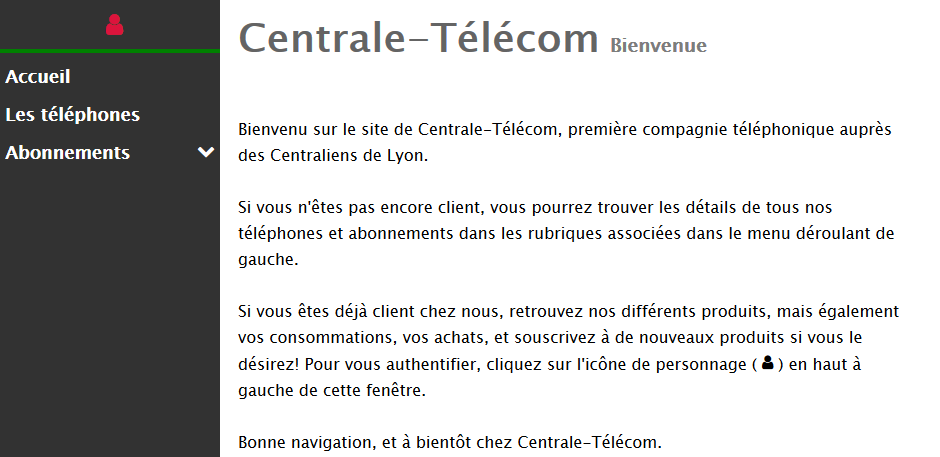
\includegraphics[width=.55\textwidth]{images/Travail_realise/hello-world}
  \caption{\'Ecran d'accueil de l'application}
  \label{fig:hello-world}
\end{figure}

%%% Local Variables:
%%% mode: latex
%%% TeX-master: "../../Rapport_BDD"
%%% End:


\section{\'Elaboration de la base de données}
\label{sec:elaboration-bdd}
\subsection{Réalisation de l'analyse Entité-Relation}

\subsubsection{Entités}

Nous avons pu identifier les entités suivantes :
\begin{itemize}
  \itemperso{Utilisateur}Chaque client doit être enregistré dans la base de données et dispose des champs suivants :
  \begin{itemize}
    \subitemperso{Nom}Son nom.
    \subitemperso{Mail}Une adresse mail.
    \subitemperso{Adresse}Une adresse pour la facturation.
    \subitemperso{Mot de passe} Un mot de passe pour l'identification lors de la connexion.
  \end{itemize}
  \itemperso{Achat}Achat d'un téléphone, d'une formule ou les deux. Ils ont chacun :
  \begin{itemize}
    \subitemperso{Date} Une date d'achat
    \subitemperso{Téléphone} Le téléphone acheté
    \subitemperso{Formule} La formule achetée
    \subitemperso{Utilisateur} L'utilisateur qui a fait l'achat
  \end{itemize}
  \itemperso{Consommation} Identifie l'ensemble des consommations effectuées par un utilisateur avec un forfait sur une période donnée.
  \begin{itemize}
    \subitemperso{Date début}Date de début de la période d'enregistrement (période de 1 mois)
    \subitemperso{Consommation Données}Le montant de données consommées sur le mobile
    \subitemperso{Achat}L'achat avec lequel a été réalisé cette consommation
  \end{itemize}
  \itemperso{SMS et MMS} Les SMS et MMS envoyés ont les propriétés suivantes :
  \begin{itemize}
    \subitemperso{Date} La date et l'heure d'envoi
    \subitemperso{Volume} Le nombre de SMS/MMS correspondant au message envoyé
    \subitemperso{Destination} Le pays de destination du SMS/MMS
    \subitemperso{Consommation} La consommation à laquelle ce message est rattaché
  \end{itemize}
  \itemperso{Appel} Les appels émis ont les propriétés suivantes :
  \begin{itemize}
    \subitemperso{Date} La date et l'heure du début de l'appel
    \subitemperso{Durée} La durée de l'appel
    \subitemperso{Destination} Le pays de destination de l'appel
    \subitemperso{Consommation} La consommation à laquelle cet appel est rattaché
  \end{itemize}
  \itemperso{Facture} Les factures des clients ont les propriétés suivantes :
  \begin{itemize}
    \subitemperso{Prix} Le montant de la facture
    \subitemperso{Payé} Si le client a payé ou non cette facture
    \subitemperso{Consommation} La consommation à laquelle cette facture est rattaché
  \end{itemize}
  \itemperso{Téléphone} Tous les modèles de téléphones en vente et leurs caractéristiques :
  \begin{itemize}
    \subitemperso{Ecran}
    \subitemperso{Technologie Internet}
    \subitemperso{TV}
    \subitemperso{Appareil Photo}
    \subitemperso{RAM}
    \subitemperso{Stockage}
    \subitemperso{Carte SD}
    \subitemperso{Double SIM}
    \subitemperso{Photo}
    \subitemperso{Modele}
    \subitemperso{Marque}
    \subitemperso{Prix}
  \end{itemize}
  \itemperso{Formule} Tous les forfaits en vente disposent de :
  \begin{itemize}
    \subitemperso{Nom} Le nom du forfait
    \subitemperso{Prix} Le prix du forfait
    \subitemperso{Limite d'appel, SMS et data} Une limite pour les sms, les appels (en durée) et les données internet (en Mo).
    \subitemperso{Plage Horaire} Plage dans laquelle les communications sont gratuites
    \subitemperso{Prix hors forfait} Différent pour les appels, les SMS et les données.
    \subitemperso{Bloqué} Si le forfait est bloqué ou non
  \end{itemize}
  \itemperso{Forfait étranger} Conditions tarifaires pour la communication vers un pays ce qui comprend les même conditions qu'une formule plus :
  \begin{itemize}
    \subitemperso{Destination} La zone géographique correspondant à ce forfait étranger
  \end{itemize}
  \itemperso{Promotion} Une promotion sur une formule
  \begin{itemize}
    \subitemperso{Prix de base}
    \subitemperso{Nouveau prix}
    \subitemperso{Téléphone} Eventuellement un autre téléphone
    \subitemperso{Date de début} Début de la promotion
    \subitemperso{Durée} Durée de la promotion
  \end{itemize}
  \itemperso{Plage Horaire} Définit une période dans la semaine
  \begin{itemize}
    \subitemperso{Nom} Nom associé à la plage horaire pour plus de clarté
    \subitemperso{Heure de début}
    \subitemperso{Heure de fin}
    \subitemperso{Jour} Les jours de la semaine concernés
  \end{itemize}
  \itemperso{Zone géographique} Définit une partie du monde
  \begin{itemize}
    \subitemperso{Nom}
  \end{itemize}
  \itemperso{Pays} Les pays du monde
  \begin{itemize}
    \subitemperso{Nom}
  \end{itemize}
\end{itemize}

\subsubsection{Les Relations}
Certaines relations 1..n ont déjà été mentionnées ci-dessus.
Les relations n..n sont les suivantes :
\begin {itemize}
  \itemperso{Formule - Plage Horaire}
  \itemperso{Forfait Etrangers - Plage Horaire}
  \itemperso{Formule - Forfait Etrangers}
  \itemperso{Formule - Téléphone}
  \itemperso{Zone Géographique - Pays}
\end {itemize}

\subsubsection{Implémentation}
Toutes les entités donneront lieu à des tables à l'exception de Promotion qui est une spécialisation de Formule. On ajoute alors les champs spécifiques à Promotion dans Formule sans toujours les utiliser.
Toutes les relations n..n donnent également lieu à des tables d'associations.


%%% Local Variables:
%%% mode: latex
%%% TeX-master: "../../Rapport_BDD"
%%% End:

\subsection{Définition des tables à utiliser}
\subsubsection{Gestion des relations \texttt{N..N}}
Pour ces relations, nous créons systématiquement une table par entité et une table de couples de clés provenant de ces tables pour réaliser la jonction entre les deux notions.

Ces tables seront mentionnées sous la forme \texttt{nom\_entité\_1\_nom\_entité\_2}.

\subsubsection{Gestion des relations \texttt{1..N}}
Pour ces relations, on créé une table par entité. De plus, pour la table provenant de l'entité ne pouvant être associé qu'à un élément de l'autre entité, on ajoute une colonne contenant la clé d'une valeur de l'autre table.

Par exemple pour entre \texttt{achat} et \texttt{formule}, on trouvera dans la table \texttt{achat} une colonne \texttt{id\_formule}.

\subsubsection{Gestion de la généralisation \texttt{isa}}
Dans le cadre de ce projet, nous avons choisi de transformer cette généralisation via une table regroupant les entités \og Formule\fg{} et \og Promotion\fg{}, mais avec des champs avec des valeurs par défaut de \texttt{-1} ou \texttt{NULL} pour différencier les éléments.

De plus, ceci nous a permis de créer des formules associées à des téléphones, ce qui a enrichi le modèle.

\subsubsection{Diagramme final}
Ainsi, nous avons en définitive aboutit au diagramme de la Figure~\ref{fig:tables}, qui présente toutes les tables proposées, ainsi que leurs liens.

La légende de cette figure est la suivante :
\begin{itemize}
  \itemperso{\bddkey}Il s'agit des clés primaires des tables. Si une table dispose de plus d'une clé primaire, alors c'est la valeur de la paire, du triplet,...qui fait office de clé primaire.
  \itemperso{\bddfkey}Il s'agit des champs utilisant la valeur d'une clé primaire d'une autre table (clé étrangère).
\end{itemize}

De plus, les tables ayant des liens entre elles (ie. utilisation de clés étrangères), sont reliés dans le schéma de la Figure~\ref{fig:tables}.

On remarquera en particulier sur cette figure, le fait que l'entité promotion ait été \og comprise\fg{} dans \texttt{formule}, avec les champs \texttt{formule\_base}, \texttt{date\_debut} et \texttt{date\_fin} qui soient pris en compte dans cette table.

Une dernière remarque concerne les champs \texttt{is\_deleted} des tables \texttt{formule} et \texttt{forfait\_etranger}. Ils ont été mis en place pour persister dans la base de données les formules n'étant plus disponibles à la vente, mais qui restent utilisées par des utilisateurs.

\begin{figure}[ht]
  \centering
  \resizebox{\textwidth}{!}{\begin{tikzpicture}[
  every matrix/.style= {minimum width=3cm, inner sep=0cm},
  every node/.style=   {inner sep=.15cm, minimum width=3cm},
  auto,
  title/.style=         {inner sep=.25cm, fill=bluenight!25},
  >=Stealth
  ]

  \matrix [minimum width=4.35cm, draw] (formule) at (0,0) [row sep=1mm,column sep=2mm]{
    \node [minimum width=4.35cm, title] (formule_name) {\textbf{Formule}};\\
    \node {\bddkey id};\\
    \node {nom};\\
    \node {prix\_mensuel};\\
    \node {limite\_appel};\\
    \node {limite\_sms};\\
    \node {limite\_data};\\
    \node {prix\_hors\_forfait\_appel};\\
    \node {prix\_hors\_forfait\_sms};\\
    \node {prix\_hors\_forfait\_data};\\
    \node {bloque};\\
    \node {prix\_base};\\
    \node {\bddfkey formule\_base};\\
    \node {date\_debut};\\
    \node {date\_fin};\\
    \node {is\_deleted};\\
  };

  \matrix [minimum width=4.35cm, below=of formule, draw] (formule_foreign) at ([yshift=-3.5cm]formule.south) [row sep=1mm,column sep=2mm]{
    \node [minimum width=4.35cm, title] (formule_foreign_name) {\textbf{Formule - Forfait étranger}};\\
    \node [minimum width=4.35cm] {\bddkey \bddfkey formule};\\
    \node [minimum width=4.35cm] {\bddkey \bddfkey forfait\_etranger};\\
  };

  \matrix [minimum width=4.35cm, right=of formule_foreign, draw] (foreign) at ([xshift=1cm]formule_foreign.east) [row sep=1mm,column sep=2mm]{
    \node [minimum width=4.35cm, title] (foreign_name) {\textbf{Forfait étranger}};\\
    \node [minimum width=4.35cm] {\bddkey id};\\
    \node [minimum width=4.35cm] {nom};\\
    \node [minimum width=4.35cm] {limite\_appel};\\
    \node [minimum width=4.35cm] {limite\_sms};\\
    \node [minimum width=4.35cm] {limite\_data};\\
    \node [minimum width=4.35cm] {prix\_hors\_forfait\_appel};\\
    \node [minimum width=4.35cm] {prix\_hors\_forfait\_sms};\\
    \node [minimum width=4.35cm] {prix\_hors\_forfait\_data};\\
    \node [minimum width=4.35cm] {bloque};\\
    \node [minimum width=4.35cm] {zone};\\
    \node [minimum width=4.35cm] {is\_deleted};\\
  };

  \matrix [right=of foreign, draw] (zone) at ([xshift=.5cm]foreign.east) [row sep=1mm,column sep=2mm]{
    \node [title] (zone_name) {\textbf{Zone géo}};\\
    \node {\bddkey id};\\
    \node {nom};\\
  };

  \matrix [above=of zone, draw] (zone_pays) at ([yshift=.5cm]zone.north) [row sep=1mm,column sep=2mm]{
    \node [title] (zone_pays_name) {\textbf{Zone géo - Pays}};\\
    \node {\bddkey \bddfkey zone\_geo};\\
    \node {\bddkey \bddfkey pays};\\
  };

  \matrix [above=of zone_pays, draw] (pays) at ([yshift=.5cm]zone_pays.north) [row sep=1mm,column sep=2mm]{
    \node [title] (pays_name) {\textbf{Pays}};\\
    \node {\bddkey id};\\
    \node {nom};\\
  };

  \matrix [above=of foreign, draw] (foreign_plage) at ([yshift=.5cm]foreign.north) [row sep=1mm,column sep=2mm]{
    \node [title] (plage_name) {\textbf{\'Etranger - Plage horaire}};\\
    \node {\bddkey \bddfkey forfait};\\
    \node {\bddkey \bddfkey plage};\\
  };

  \matrix [above=of foreign_plage, draw] (plage) at ([yshift=.5cm]foreign_plage.north) [row sep=1mm,column sep=2mm]{
    \node [title] (plage_name) {\textbf{Plage horaire}};\\
    \node {\bddkey id};\\
    \node {nom};\\
    \node {heure\_debut};\\
    \node {heure\_fin};\\
    \node {jour};\\
  };

  \path
  let \p1 = (formule.north),
      \p2 = (plage.north)
  in coordinate (whereformuleplage) at ({(\x1+\x2)/2},{\y1+2});

  \matrix [above=of formule, draw] (formule_plage) at (whereformuleplage) [row sep=1mm,column sep=2mm]{
    \node [title] (formule_plage_name) {\textbf{Formule - Plage horaire}};\\
    \node {\bddkey \bddfkey formule};\\
    \node {\bddkey \bddfkey plage\_horaire};\\
  };

  \matrix [left=of formule, draw] (achat) at ([xshift=-1cm]formule.west) [row sep=1mm,column sep=2mm]{
    \node [title, minimum width=3.5cm] (achat_name) {\textbf{Achat}};\\
    \node [minimum width=3.5cm] {\bddkey idachat};\\
    \node [minimum width=3.5cm] {date};\\
    \node [minimum width=3.5cm] {\bddfkey telephone};\\
    \node [minimum width=3.5cm] {\bddfkey id\_utilisateur};\\
    \node [minimum width=3.5cm] {\bddfkey id\_formule};\\
  };

  \matrix [above=of achat, draw] (user) at ([yshift=1cm]achat.north) [row sep=1mm,column sep=2mm]{
    \node [title] (user_name) {\textbf{Utilisateur}};\\
    \node {\bddkey idutilisateur};\\
    \node {nom};\\
    \node {mail};\\
    \node {adresse};\\
    \node {mot\_de\_passe};\\
    \node {admin};\\
  };

  \matrix [minimum width=3.3cm, left=of formule, draw] (phone) at ([xshift=-5cm, yshift=-3cm]formule.south west) [row sep=1mm,column sep=2mm]{
    \node [title, minimum width=3.3cm] (phone_name) {\textbf{Téléphone}};\\
    \node {\bddkey idtelephone};\\
    \node {écran};\\
    \node {tv};\\
    \node {appareil\_photo};\\
    \node {vidéo\_numérique};\\
    \node {ram};\\
    \node {carte\_sd};\\
    \node {double\_sim};\\
    \node {photo\_url};\\
    \node {modele};\\
    \node {marque};\\
    \node {prix};\\
    \node {stockage};\\
    \node {capacité\_internet};\\
  };

  \path
  let \p1 = (phone.north),
      \p2 = (formule.west),
      \p3 = (phone.east)
  in coordinate (wherephoneassoc) at ({(\x3+\x2)/2},\y1);

  \matrix [minimum width=4.35cm, anchor=north, draw] (formule_phone) at (wherephoneassoc) [row sep=1mm,column sep=2mm]{
    \node [minimum width=4.35cm, title] (formule_phone_name) {\textbf{Formule - Téléphone}};\\
    \node [minimum width=4.35cm] {\bddkey \bddfkey formule};\\
    \node [minimum width=4.35cm] {\bddkey \bddfkey telephone};\\
  };

  \matrix [left=of user, draw] (mms) at ([xshift=-.5cm]user.west) [row sep=1mm,column sep=2mm]{
    \node [title, minimum width=3.5cm] (mms_name) {\textbf{MMS}};\\
    \node [minimum width=3.5cm] {\bddkey idmms};\\
    \node [minimum width=3.5cm] {volume};\\
    \node [minimum width=3.5cm] {date};\\
    \node [minimum width=3.5cm] {\bddfkey destination};\\
    \node [minimum width=3.5cm] {\bddfkey consommation};\\
  };

  \matrix [left=of mms, draw] (sms) at ([xshift=-.5cm]mms.west) [row sep=1mm,column sep=2mm]{
    \node [title, minimum width=3.5cm] (sms_name) {\textbf{SMS}};\\
    \node [minimum width=3.5cm] {\bddkey idsms};\\
    \node [minimum width=3.5cm] {volume};\\
    \node [minimum width=3.5cm] {date};\\
    \node [minimum width=3.5cm] {\bddfkey destination};\\
    \node [minimum width=3.5cm] {\bddfkey consommation};\\
  };

  \matrix [left=of sms, draw] (appel) at ([xshift=-.5cm]sms.west) [row sep=1mm,column sep=2mm]{
    \node [title, minimum width=3.5cm] (appel_name) {\textbf{Appel}};\\
    \node [minimum width=3.5cm] {\bddkey idappel};\\
    \node [minimum width=3.5cm] {debut\_appel};\\
    \node [minimum width=3.5cm] {duree};\\
    \node [minimum width=3.5cm] {\bddfkey destination};\\
    \node [minimum width=3.5cm] {\bddfkey consommation};\\
  };

  \path
  let \p1 = (achat.west),
      \p2 = (sms.south)
  in coordinate (whereconso) at (\x2,\y1);

  \matrix [draw] (conso) at (whereconso) [row sep=1mm,column sep=2mm]{
    \node [title, minimum width=3.8cm] (conso_name) {\textbf{Consommation}};\\
    \node [minimum width=3.8cm] {\bddkey idconsommation};\\
    \node [minimum width=3.8cm] {date\_début};\\
    \node [minimum width=3.8cm] {conso\_data};\\
    \node [minimum width=3.8cm] {\bddfkey id\_achat};\\
  };

  \matrix [below=of conso, draw] (facture) at ([yshift=-.5cm]conso.south) [row sep=1mm,column sep=2mm]{
    \node [title, minimum width=3.5cm] (facture_name) {\textbf{Facture}};\\
    \node [minimum width=3.5cm] {\bddkey idfacture};\\
    \node [minimum width=3.5cm] {\bddfkey consommation};\\
    \node [minimum width=3.5cm] {prix};\\
    \node [minimum width=3.5cm] {payé};\\
  };

  \draw let \p0 = (formule.north), \p1 = (formule_plage.west) in (\x0,\y0) -- (\x0,\y1) -- (\x1,\y1);
  \draw let \p0 = (formule_plage.east), \p1 = (plage.north) in (\x0,\y0) -- (\x1,\y0) -- (\x1,\y1);
  \draw let \p1 = (conso.east), \p2 = (achat.west) in (\x1,\y2) -- (\x2,\y2);
  \draw let \p1 = ([yshift=-.5cm]conso.north west), \p2 = (appel.south) in (\x1,\y1) -- (\x2,\y1) -- (\x2,\y2);
  \draw let \p1 = ([yshift=-.7cm]conso.north east), \p2 = (mms.south) in (\x1,\y1) -- (\x2,\y1) -- (\x2,\y2);

  \draw (foreign.east) -- (zone.west);
  \draw (zone.north) -- (zone_pays.south);
  \draw (zone_pays.north) -- (pays.south);
  \draw (achat.east) -- (formule.west);
  \draw let \p1 = ([yshift=.5cm]achat.south west), \p2 = (phone.north) in (\x1,\y1) -- (\x2,\y1) -- (\x2,\y2);
  \draw (user.south) -- (achat.north);
  \draw (facture.north) --  (conso.south);
  \draw (conso.north) -- (sms.south);
  \draw (foreign.north) -- (foreign_plage.south);
  \draw (foreign_plage.north) -- (plage.south);
  \draw let \p0=([yshift=2cm]appel.north), \p1=([xshift=.75cm]pays.north) in (appel.north) -- (\x0,\y0) -- (\x1,\y0) -- (\x1,\y1);
  \draw let \p0=([yshift=1.75cm]sms.north), \p1=(pays.north) in (sms.north) -- (\x0,\y0) -- (\x1,\y0) -- (\x1,\y1);
  \draw let \p0=([yshift=1.5cm]mms.north), \p1=([xshift=-.75cm]pays.north) in (mms.north) -- (\x0,\y0) -- (\x1,\y0) -- (\x1,\y1);
  \draw (formule.south) -- (formule_foreign.north);
  \draw (formule_foreign.east) -- (foreign.west);
  \draw let \p0=(formule_phone.west), \p1=(phone.east) in (\x0,\y0) -- (\x1,\y0);
  \draw let \p0=(formule_phone.east), \p1=(formule.west) in (\x0,\y0) -- (\x1,\y0);
\end{tikzpicture}

%%% Local Variables:
%%% mode: latex
%%% TeX-master: "../../Rapport_BDD"
%%% End:
}
  \caption{Relations entre les tables de la base de données}
  \label{fig:tables}
\end{figure}


%%% Local Variables:
%%% mode: latex
%%% TeX-master: "../../Rapport_BDD"
%%% End:


\section{Plateforme réalisée}
\textit{Nous détaillerons dans cette partie les différents visuels de la plateforme. Nous préciserons également le fonctionnement administratif de la plateforme (clients, administrateurs, visiteurs).}
\subsection{Les différentes vues}
\subsubsection{Liste des vues}
La plateforme est organisée selon une architecture MVC (Modèle - Vue - Contrôleur). Ainsi, les différents visuels/pages proposés (les vues) sont chacuns représentés par un fichier. Dans notre cas, ces fichiers sont situés dans le répertoire \texttt{telephonie/vue}. Nous allons dans un premier temps détailler la liste des vues, ces dernières seront ensuite présentées (fonctionnement et interraction avec les utilisateurs) dans les sous-sections suivantes.

Ainsi, l'application proposé au total sept vues :
\begin{itemize}
  \itemperso{Accueil}La page d'arrivée dans l'application qui présente uniquement les principaux objectifs de ce dernier. Ce visuel vous a été présenté à la Figure~\ref{fig:hello-world}.
  \itemperso{Téléphones}Cette page présente les différents téléphones proposés à la vente par Cenrale-Télécom. Elle permet au client de s'informer sur les modèles et de les acheter. Dans le même temps, elle permet à l'équipe administrative d'en référencer de nouveaux.
  \itemperso{Compte/Utilisateur}Ces vues permettent soit l'administration des utilisateurs par les administrateurs, soit à un client donné de consulter ses informations et de changer ses informations.
  \itemperso{Connexion}Une vue permet aux utilisateurs de se connecter/déconnecter.
  \itemperso{Factures}Cette vue n'est accessible qu'aux clients et permet à ces derniers de consulter leurs factures et de télécharger cette dernière au format PDF.
  \itemperso{Abonnements}Cette vue se décompose en trois vues intermédiaires :
  \begin{itemize}
    \subitemperso{Mes abonnements}Cette vue permet à un client de retrouver tous les abonnements auxquels il a souscrit, ainsi que les téléphones achetés chez Centrale-Télécom.
    \subitemperso{Vers l'étranger}Cette vue permet de préciser tous les abonnements étrangers proposés par Centrale-Télécom. Elle permet également aux administrateurs d'ajouter de nouveaux forfaits.
    \subitemperso{Formules}Cette vue permet de préciser toutes les formules proposées par Centrale-Télécom. Elle permet également aux administrateurs d'ajouter de nouvelles formules.
  \end{itemize}
\end{itemize}
Les spécificités par utilisateurs seront précisées plus en détails dans les sous-sections suivantes, ainsi que toutes les actions possibles.

\subsubsection{Navigation dans l'application}
Le dernier point général sur cette application est la navigation. Cette dernière est facilitée par un panneau latéral qui présente tous les menus de l'application. Dans le cas d'un client \og lambda\fg{}, on dispose du panneau latéral observable à la Figure~\ref{fig:navigation}.

\begin{figure}[ht]
  \centering
  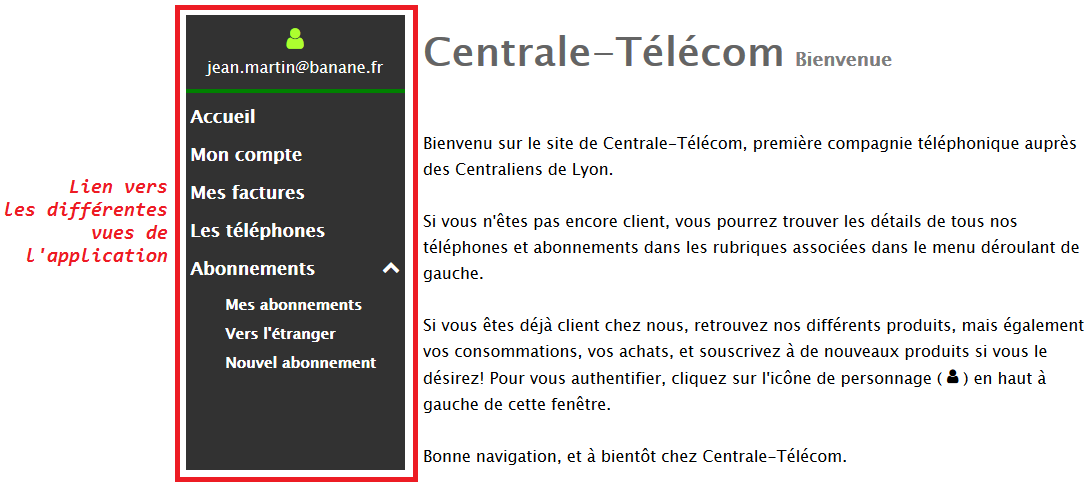
\includegraphics[width=.55\textwidth]{images/Plateforme/navigation}
  \caption{Panneau de navigation pour l'application}
  \label{fig:navigation}
\end{figure}

À moins d'être à l'accuel (cas de la Figure~\ref{fig:navigation}), la page courrante est surligné dans le volet de navigation pour que les utilisateurs sachent où ils se situent dans l'application.

%%% Local Variables:
%%% mode: latex
%%% TeX-master: "../../Rapport_BDD"
%%% End:

\subsection{Gestion des utilisateurs}
\subsubsection{Les différents types d'utilisateurs}
L'application est structurée autours de trois niveaux hiérarchiques pour les utilisateurs :
\begin{itemize}
  \itemperso{Visiteur}Il s'agit du niveau avec le moins d'accréditations possibles. Cet utilisateur correspond à une personne lambda naviguant sur le site, sans être client de Centrale-Télécom.
  \itemperso{Client}Ce niveau permet de représenter les clients qui viennent consulter leurs factures, leurs abonnements ou encore les nouvelles offres disponibles.
  \itemperso{Administrateur}Ce grade est celui avec le plus de droit. Il représente les employés de Centrale-Télécom qui ont donc le droit d'éditer les profils, créer des abonnements, des téléphones,...
\end{itemize}
Les clients et les administrateurs sont des profils qui sont détectés après une connexion à la plateforme. Ils sont différenciés au niveau de la base de données via la colonne \texttt{admin} de la table \texttt{utilisateur}, qui est mise à \texttt{TRUE} si l'utilisateur est un administrateur. Une fois la connexion effectuée, on stocke les informations dans la variable globale \texttt{\$\_SESSION}. Le cas des visiteurs correspond alors aux valeurs par défaut pour \texttt{\$\_SESSION}. On retrouve alors les caractéristiques de la Table~\ref{tab:utilisation_session}.

\begin{table}[ht]
  \centering
  \begin{tabular}{ccc}
    \toprule
    \textbf{Type d'utilisateur} & \textbf{Champ \texttt{log\_in}} & \textbf{Champ \texttt{login\_level}} \\
    \midrule
    Visiteur & \texttt{False} & Sans importance (\texttt{False}) \\
    Client   & \texttt{True} & \texttt{False} \\
    Administrateur & \texttt{True} & \texttt{True} \\
    \bottomrule
  \end{tabular}
  \caption{Valeurs stockées dans \texttt{\$\_SESSION} pour les différents profils d'utilisateurs}
  \label{tab:utilisation_session}
\end{table}

Ces grandeurs nous permettent d'adapter les affichages en fonction du type d'utilisateur.

\subsubsection{Connexion et déconnexion}
\subParagraphe{Réalisation des actions}Ces deux actions sont réalisées à partir d'un vue accesible en cliquant sur l'icône \thColor{\faUser}.

\begin{figure}[ht]
  \centering
  \begin{subfigure}{.45\textwidth}
    \centering
    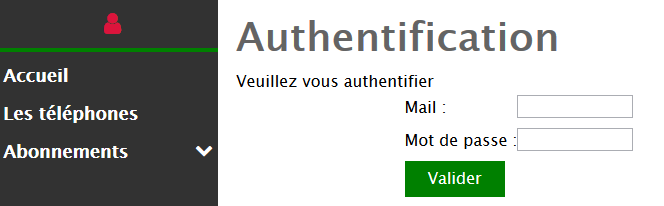
\includegraphics[width=.95\textwidth]{images/Plateforme/connexion}
    \caption{Connexion d'un utilisateur}
    \label{fig:connexion}
  \end{subfigure}\hfill%
  \begin{subfigure}{.45\textwidth}
    \centering
    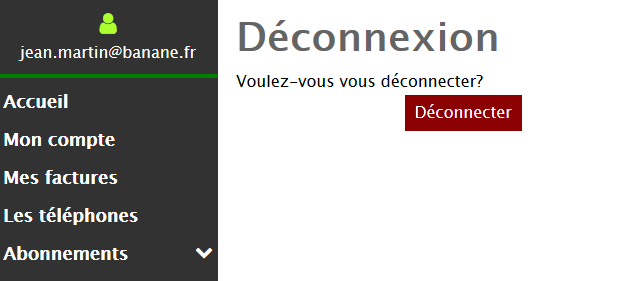
\includegraphics[width=.95\textwidth]{images/Plateforme/deconnexion}
    \caption{Déconnexion d'un utilisateur}
    \label{fig:deconnexion}
  \end{subfigure}
  \caption{Les fenêtres de connexion et déconnexion des utilisateurs}
\end{figure}

Une première vue (Figure~\ref{fig:connexion}) permet aux utilisateurs de se déconnecter. Le principe est usuel, où l'utilisateur va fournir son adresse mail (qui fait office d'identifiant ici) ainsi que son mot de passe. Si les deux concordent, l'utilisateur est connecté, sinon il devra ré-essayer.

Pour la déconnexion, il suffit de se rendre aussi sur cette page (Figure~\ref{fig:deconnexion}), qui propose alors un bouton pour se déconnecter.

\subParagraphe{Différences visuelles}On remarquera également une différence sur la partie haute de la barre de navigation, où l'avatar \faUser{} est en rouge (\thColor{\faUser}) si l'utilisateur n'est pas enregistré et en vert (\textcolor{vertforet}{\faUser}) si l'utilisateur est connecté. De même, quand l'utilisateur est connecté, son adresse mail apparaît sous cette icône.

\subParagraphe{Pour les visiteurs}Un visiteur ne disposant pas de compte, il ne peut se connecter, et n'aura donc accès à aucune vue de celles précisées dans la suite de cette section.

\subsubsection{\'Edition du profil en tant que client}
Un client dispose de la possibilité de voir et éditer les informations de son profil (sauf son statut!) directement par la vue intitulée \og Mon compte\fg. La vue de consultation du profil vous est proposée à la Figure~\ref{fig:vueprofilclient} présente les différentes informations au client, ainsi qu'un bouton d'édition. La vue d'édition associée est présentée à la Figure~\ref{fig:vueeditionclient}.

\begin{figure}[ht]
  \centering
  \begin{subfigure}{.45\textwidth}
    \centering
    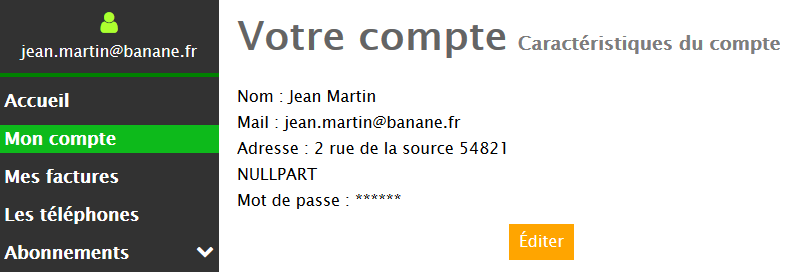
\includegraphics[width=.95\textwidth]{images/Plateforme/vue_profil_client}
    \caption{Vue du profil}
    \label{fig:vueprofilclient}
  \end{subfigure}\hfill%
  \begin{subfigure}{.45\textwidth}
    \centering
    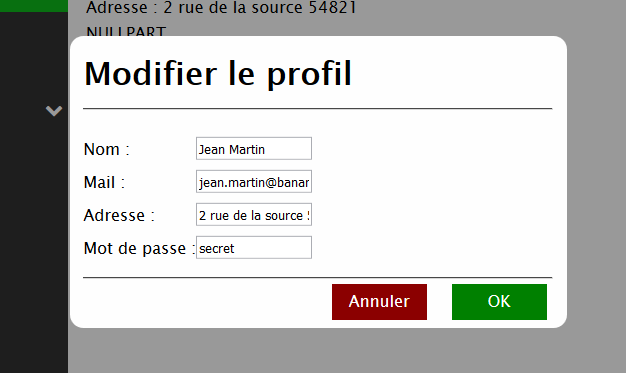
\includegraphics[width=.95\textwidth]{images/Plateforme/vue_edition_profil}
    \caption{\'Edition de son profil}
    \label{fig:vueeditionclient}
  \end{subfigure}
  \caption{Gestion du compte par un client}
\end{figure}

\subsubsection{\'Edition des profils en tant qu'administrateur}
Un administrateur dispose lui de plus de droit. Il peut ainsi voir la liste de tous les utilisateurs inscrits à la plateforme, qu'ils soient administrateurs ou simples clients. On remarquera cependant qu'un administrateur qui consulte cette liste ne peut se voir lui-même, pour éviter une modification involontaire de son profil. Cette vue vous est proposée à la Figure~\ref{fig:listeusers}

\begin{figure}[ht]
  \centering
  \begin{subfigure}{.65\textwidth}
    \centering
    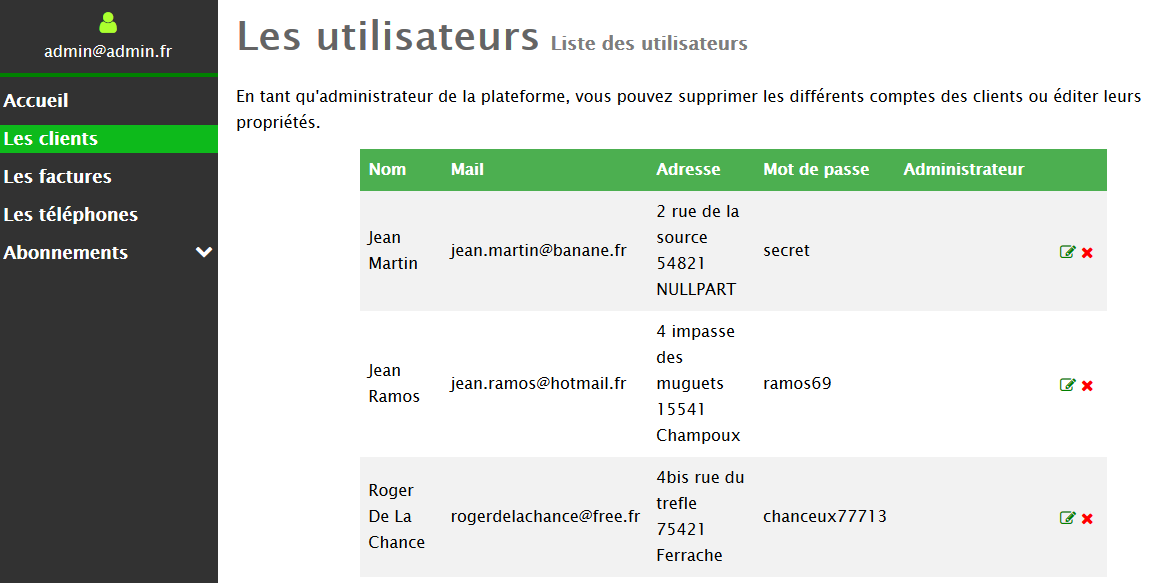
\includegraphics[width=.95\textwidth]{images/Plateforme/liste_utilisateurs}
    \caption{Liste des clients}
    \label{fig:listeusers}
  \end{subfigure}\hfill%
  \begin{subfigure}{.35\textwidth}
    \centering
    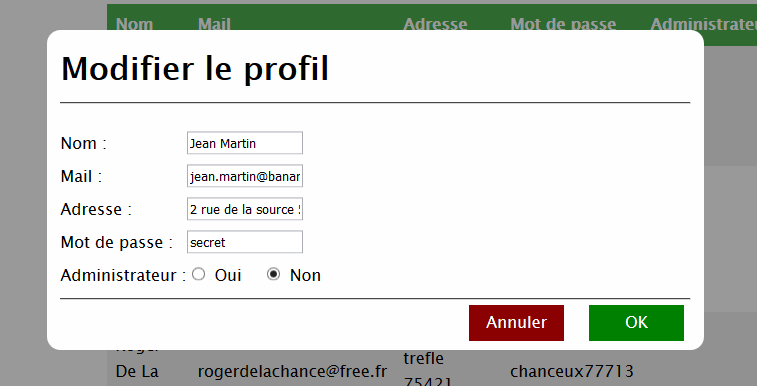
\includegraphics[width=.95\textwidth]{images/Plateforme/vue_edition_clients}
    \caption{\'Edition d'un utilisateur}
    \label{fig:editionuser}
  \end{subfigure}
  \caption{Gestion des comptes clients par un administrateur}
\end{figure}

En effet, outre la liste des utilisateurs, l'administrateur dispose du droit de modifier tous les comptes, que ce soit pour les adresses mails, les noms, les mots de passe ou encore les droits d'accès à la plateforme (administrateur ou non). La fenêtre d'édition est précisée à la Figure~\ref{fig:editionuser} et s'ouvre en cliquant sur une icône \vColor{\faEdit}.

Enfin, l'administrateur peut également supprimer des comptes clients en cliquant sur l'icône \thColor{\faRemove}. On remarquera que dans cette vue, des informations sont apportées à l'administrateur en cas d'échec ou de réussite de sa manipulation.

%%% Local Variables:
%%% mode: latex
%%% TeX-master: "../../Rapport_BDD"
%%% End:

\subsection{Les téléphones}
Cette partie permet de voir la liste des téléphones, éditer leurs configurations et les acheter.

\subsubsection{Consulter la liste des téléphones}
Cette action est disponible pour tous les types d'utilisateurs. Pour cela, il suffit de cliquer sur la lignes \og Les téléphones\fg{} de la barre de menu. On aboutit alors à l'interface de la Figure~\ref{fig:phones-list}.

\begin{figure}[ht]
  \centering
  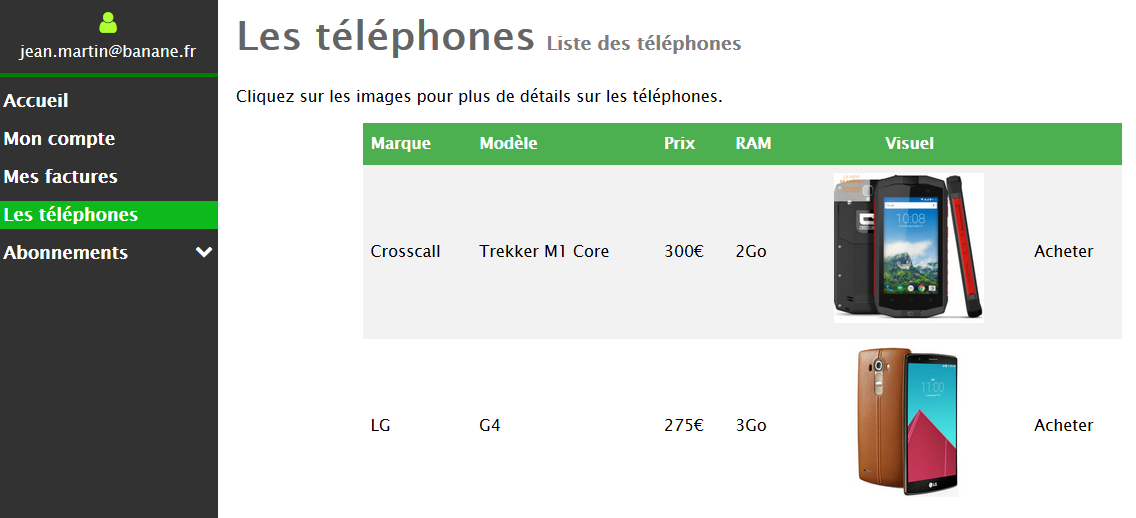
\includegraphics[width=.7\textwidth]{images/Plateforme/phone-list}
  \caption{Consulter la liste des téléphones}
  \label{fig:phones-list}
\end{figure}

On remarquera que cette liste ne propose pas initialement toutes les caractéristiques des téléphones. Afin d'accéder à ces dernières, l'utilisateur doit cliquer sur l'image du téléphone. Une modale avec tous les détails apparaît alors, comme proposée à la Figure~\ref{fig:phone-details}.

\begin{figure}[ht]
  \centering
  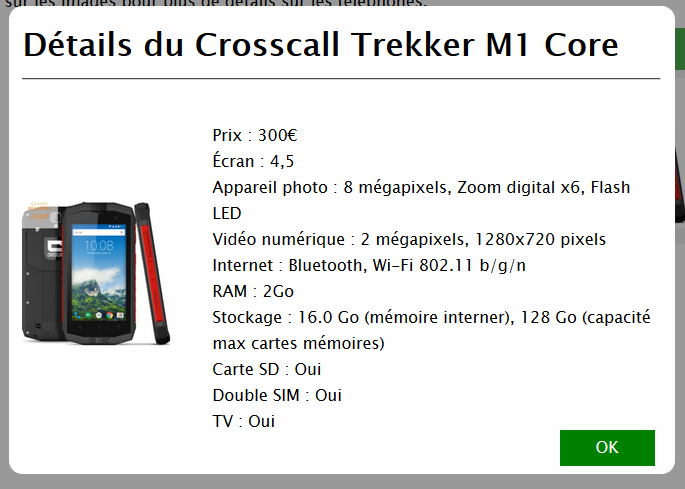
\includegraphics[width=.7\textwidth]{images/Plateforme/phone-details}
  \caption{Affichage des détails d'un téléphone}
  \label{fig:phones-details}
\end{figure}

\subsubsection{Créer et modifier un téléphone}
Ces actions ne peuvent être réalisées que par un administrateur.
\subParagraphe{Créer un nouveau téléphone}Pour cela, un administrateur doit simplement cliquer sur le bouton \og Nouvel appareil\fg. Une modale s'ouvre alors, lui proposant de remplir tous les champs permettant de caractériser le téléphone. Cette modale vous est proposée à la Figure~\ref{fig:new-phone}.

\begin{figure}[ht]
  \centering
  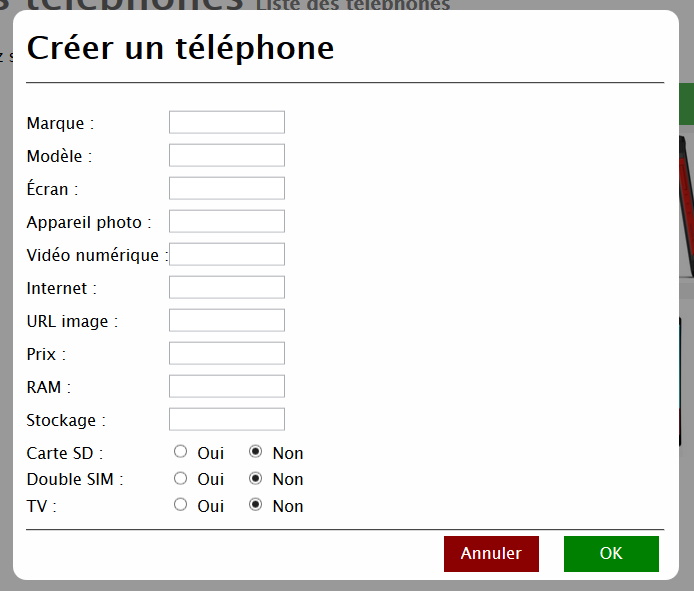
\includegraphics[width=.5\textwidth]{images/Plateforme/new_phone}
  \caption{Création d'un téléphone}
  \label{fig:new-phone}
\end{figure}

Si en cliquant sur \og OK\fg, la table n'est pas mis à jour, c'est que certains champs obligatoires n'ont pas été remplis. Sinon, tous les champs remplis sont corrects.

\subParagraphe{\'Edition d'un téléphone}De manière transparente, l'administrateur peut cliquer sur l'icône \vColor{\faEdit} d'un téléphone. Une modale de même aspect que celle de la Figure~\ref{fig:new-phone} apparaît alors avec les valeurs pré-remplies du téléphone. L'administrateur peut alors éditer ces valeurs à loisir.

\subParagraphe{Suppresion d'un téléphone}Cette dernière se fait en cliquant sur l'icône \thColor{\faRemove} du téléphone. Ce dernier n'est alors pas supprimé entièrement de la base de données. Il est supprimé des formules qui le proposait auparavant, et son champ \texttt{is\_deleted} qui représente sa mise sur le marché est mis à \texttt{TRUE}, pour que ce dernier n'apparaisse plus dans les listes de téléphones. Il n'est cependant pas totalement supprimé de la base de données, pour que les utilisateurs l'ayant acheté le voit toujours apparaître dans leur liste d'achat.

\subsubsection{Achter un téléphone}
Cette action ne peut être réalisée que par un client. Pour cela, ce dernier dispose de la possibilité de cliquer sur la case \og Acheter\fg{} à la fin de chaque ligne de la table présentant les téléphones. En faisant ainsi, une modale s'ouvre pour valider la commande, comme présentée à la Figure~\ref{fig:achat-phone}.

\begin{figure}[ht]
  \centering
  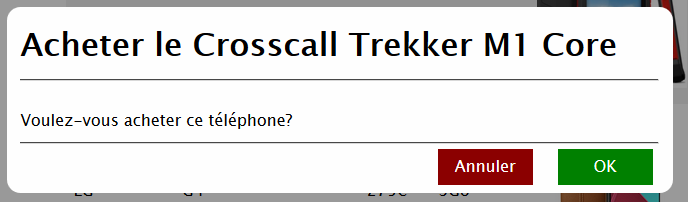
\includegraphics[width=.6\textwidth]{images/Plateforme/buy_phone}
  \caption{Confirmation de l'achat d'un téléphone}
  \label{fig:achat-phone}
\end{figure}

En cliquant sur \og OK\fg, le client valide alors la commande, il peut annuler l'action en cliquant sur \og Annuler\fg. La consultation de la liste des téléphones achetés sera détaillée plus loin dans la partie consacrée aux abonnements.



%%% Local Variables:
%%% mode: latex
%%% TeX-master: "../../Rapport_BDD"
%%% End:

\subsection{Consultation des factures}
Cette section concerne la création et la consultation de factures ainsi que la génération des détails de consommation de chaque utilisateur sous forme d'un fichier PDF.
\subsubsection{Liste des factures}
Lors que l'utilisateur identifié clique sur la section \og Les factures\fg il voit alors apparaitre la liste de ses factures dans un tableau ressemblant à celui présent sur la Figure~\ref{fig:listfacture}

\begin{figure}[ht]
  \centering
    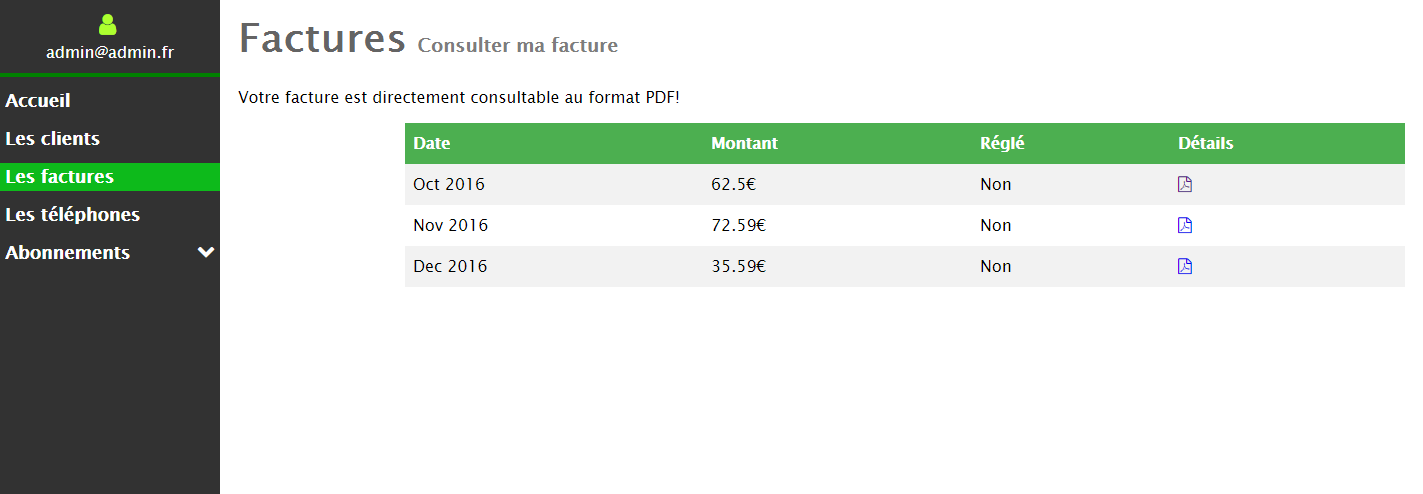
\includegraphics[width=.55\textwidth]{images/Plateforme/liste_factures}
    \caption{Liste des factures}
    \label{fig:listfacture}
\end{figure}

Les champs de ce tableau sont les suivants :
\begin{itemize}
  \itemperso{Date}Le mois de facturation : correspond à la période pendant laquelle les opérations téléphoniques ont eu lieu.
  \itemperso{Montant}Le montant de la facture à payer en euros.
  \itemperso{Reglé}\og Oui\fg si la facture est déjà payée, \og Non\fg sinon.
  \itemperso{Détails}Un lien vers une page qui génère et affiche le détails des consommations de l'utilisateur pour le mois sélectionné.
\end{itemize}

\subsubsection{Détail des consommations}

Le PDF généré donne les consommations détaillées de l'utilisateur pour trois types de consommations différentes :
\begin{itemize}
	\itemperso{SMS}Présenté en Figure~\ref{fig:liste_sms_pdf}
	\itemperso{MMS}Présenté en Figure~\ref{fig:liste_mms_pdf}
	\itemperso{appel}Présenté en Figure~\ref{fig:liste_appels_pdf}
\end{itemize}

\begin{figure}[ht]
  \begin{subfigure}{.33\textwidth}
    \centering
    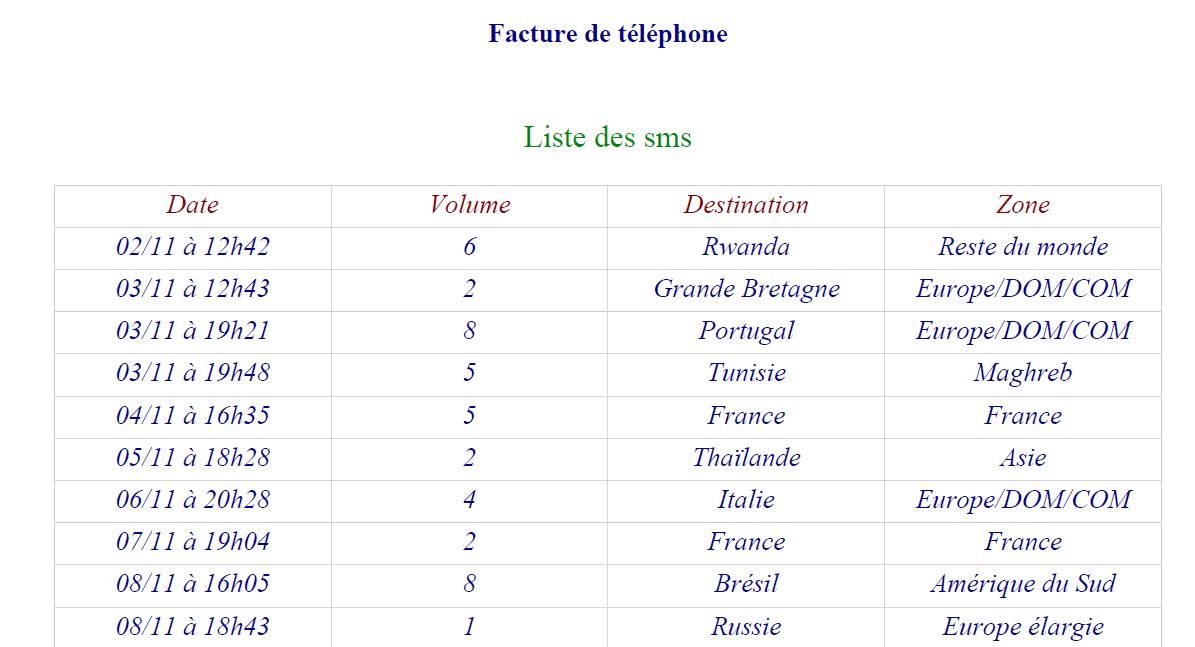
\includegraphics[width=\textwidth]{images/Plateforme/liste_sms_pdf}
    \caption{Liste des SMS}
    \label{fig:liste_sms_pdf}
  \end{subfigure}\hfill%
  \begin{subfigure}{.33\textwidth}
    \centering
    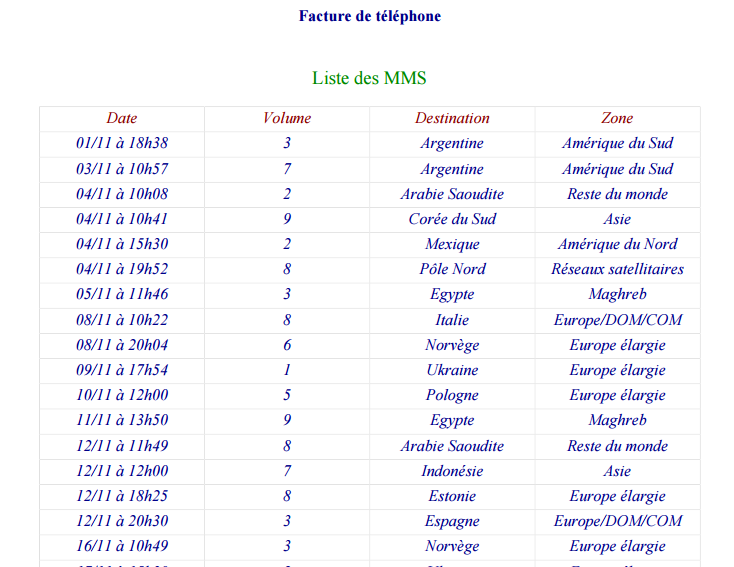
\includegraphics[width=\textwidth]{images/Plateforme/liste_mms_pdf}
    \caption{Liste des MMS}
    \label{fig:liste_mms_pdf}
  \end{subfigure}\hfill
  \begin{subfigure}{.33\textwidth}
    \centering
    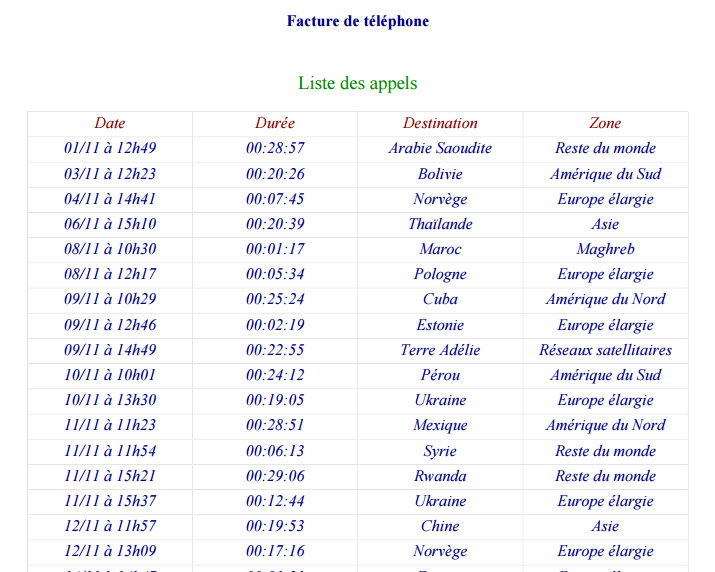
\includegraphics[width=\textwidth]{images/Plateforme/liste_appels_pdf}
    \caption{Liste des appels}
    \label{fig:liste_appels_pdf}
  \end{subfigure}
  \caption{Listes générées dans le PDF}
\end{figure}


%%% Local Variables:
%%% mode: latex
%%% TeX-master: "../../Rapport_BDD"
%%% End:

\subsection{Gestion des abonnements}
Cette partie va présenter toutes les fonctionnalités relatives à la consultation, la modification et la souscription à un abonnement. Du point de vue des utilisateurs, tous (y compris les visiteurs) ont accès à la consultation des offres (formules et forfaits étrangers). Par contre, un client à accès en plus à un résumé de ses achats (téléphone et formules).

\subsubsection{La liste des formules}
Cette vue est la principale associée à la gestion des abonnements. Elle présente un résumé de la liste des formules proposés par Centrale-Télécom. Le tableau présente donc les principales caractéristiques des formules, à savoir :
\begin{itemize}
  \itemperso{Nom et tarif}Les informations basiques pour que les utilisateurs se repèrent dans les formules.
  \itemperso{Promotion}Cette valeur est mise à \og Oui\fg{} si la formule est une promotion, \og Non\fg{} sinon.
  \itemperso{Téléphone associé}L'icône permet de savoir si la formule est associée à un ou plusieurs téléphones. Ceci permet de représenter les liens (par exemples promotionnels) entre une formule et un téléphone. Si un ou deux téléphones sont associés, alors l'icône est \vColor{\faMobilePhone}, sinon il s'agit de \thColor{\faMobilePhone}.
  \itemperso{Forfaits étrangers}Tout comme le champs sur les téléphones, il permet de savoir si l'offre est associée à une formule vers l'étranger. Ici aussi, si un ou plusieurs forfaits étrangers sont inclus dans la formule, alors l'icône est \vColor{\faGlobe}, sinon il s'agit de \thColor{\faGlobe}.
  \itemperso{Boutons d'édition}
\end{itemize}
Ces différents éléments peuvent être observés à la Figure~\ref{fig:}


%%% Local Variables:
%%% mode: latex
%%% TeX-master: "../../Rapport_BDD"
%%% End:


\section{Aspects techniques de la plateforme}
\subsection{Architecture de la plateforme}

\subsubsection{Architecture MVC}
La plateforme a été réalisée en ayant pour volonter de mettre en place une architecture MVC minimale.

Pour cela, le code a été organisé selon trois dossiers principaux :
\begin{itemize}
  \itemperso{\texttt{controleur}}Ce fichier contient tous les contrôleurs associés au modèle.
  \itemperso{\texttt{vue}}Ce fichier contient toutes les vues du site, ie. des visuels qui réutilisent des informations calculées par les contrôleurs.
  \itemperso{\texttt{database}}Normalement, le fichier aurait dû être appelé \texttt{modèle} dans une architecture MVC classique, cependant, toutes les opérations liées au modèle sont presque exclusivement réalisées en SQL dans cette application, ce fichier a donc \og pris sa place\fg.
\end{itemize}
Dans la suite, nous allons préciser comment les ressources sont chargées pour chaque page.

\subsubsection{Appel des vues}
\subParagraphe{Charger les fichiers}Le centre de l'architecture mise en place est le fichier \texttt{index.php}. Ce dernier réalise toutes les inclusions nécessaires en PHP, via les commandes :

\begin{lstlisting}[language=php]
  require 'database/DB.php';
  require 'controleur/users_controller.php';
  require 'controleur/bills_controller.php';
  require 'vue/vue.php';
  .../...
\end{lstlisting}

\subParagraphe{Création d'une vue}Ensuite, nous créons dans ce fichier une vue (instance de l'objet \texttt{Vue}). Cet instance permettra d'afficher les éléments dans la page.

\subParagraphe{Assignation de la vue à un contrôleur}Enfin, le fichier va récupérer via les paramètres passés dans l'URL, le nom de la vue qui est demandée. En fonction du résultat, il va créer le contrôleur associé à la vue. Ceci est réalisée par le \texttt{swicth} suivant :

\begin{lstlisting}[language=php]
  if (isset($_GET['vue'])){
    switch($_GET['vue']){
      case 'users':
        $controleur = new UsersController($vue, $_SESSION['log_in'], $_SESSION['login_level']);
        break;
      case 'bills':
        $controleur = new BillsController($vue, $_SESSION['log_in'], $_SESSION['login_level']);
        break;
      case .../...
\end{lstlisting}

Ainsi, chaque contrôleur est crée avec la vue pour l'afficher en paramètre. Chaque contrôleur va alors appeler spécifiquement son affichage via des commandes de la forme :

\begin{lstlisting}[language=php]
  function __construct($vue)  {
    $vue->display('bills', 'Factures', 'Consulter ma facture', $this);
  }
\end{lstlisting}
% $

\subParagraphe{Récupération du fichier spécifique à la vue}Enfin, la dernière étape revient à charger le fichier de la vue associée au contrôleur (et non plus la classe \texttt{Vue}). Pour cela, l'instance \texttt{\$vue} dispose d'une méthode \texttt{determine\_vue} qui est appelée par \texttt{display} et qui contient les associations entre les vues demandées et leur fichier associé.

\subParagraphe{Relancer le processus}Ce processus sera relancé à partir de la recherche du contrôleur dès que le client clique sur un des liens du panneau latéral.

\subsubsection{Les fichiers affichés}
Comme nous l'avons évoqué, les fichiers affichés sont situés dans le répertoire \texttt{vue}. De manière plus précise, le fichier contenant la bare latéral de navigation et qui est affiché quelle que soit la situation est nommé \texttt{main.html.php}. Tous les autres fichiers ont des noms relatifs aux objets donc ils sont les vues. Ainsi, \texttt{phone.html.php} correspond par exemple à la vue pour les téléphones.

Comme cela a été expliqué, toutes les correspondances sont visibles dans le fichier \texttt{vue.php} qui contient la classe \texttt{Vue}.

\subsubsection{Scripts, styles et autres éléments}
\subParagraphe{Feuilles de style}Les feuilles de styles de l'application sont stockées dans le dossier \texttt{assets/styles}.
\subParagraphe{Scripts JS}Les scripts Javascript utilisés pour l'application sont stockées dans le dossier \texttt{assets/scripts}.
\subParagraphe{Polices}L'application utilise avec parcimonie la police Font Awesome pour afficher des éléments graphiques (\faChevronDown, \faUser, \faRemove,...). Cette police est contenue dans le dossier \texttt{assets/fonts}.
\subParagraphe{Fichiers XSL et XML}Ces fichiers utilisés pour la génération du PDF (voir Section~\ref{sec:pdf}) sont directement disposés dans le dossier \texttt{vue}, car directement liés à ces dernières.

%%% Local Variables:
%%% mode: latex
%%% TeX-master: "../../Rapport_BDD"
%%% End:

\subsection{Connexion à la base de données}
La connexion à la base de données est réalisée par la classe \texttt{DB}. Cette classe offre les fonctionnalités discutées dans cette section.

\subsubsection{Connexion et déconnexion}
La connexion est réalisée dans le constructeur, en utilisant \texttt{mysqli}. En particulier, les lignes suivantes permettent de configurer la connexion à la base de données et sont à adapter à votre propre cas :

\begin{lstlisting}[language=php]
  $this->servername = "localhost";
  $this->username = "root";
  $this->password = "0000";
  $this->dbname = "telephonie";
\end{lstlisting}

En cas d'erreur, cette classe renvoie une erreur pour avertir l'utilisateur que la connexion a échouée.

La déconnexion est assurée via la méthode \texttt{close}.

\subsubsection{Exécution de requête}
Pour exécuter des requêtes, deux méthodes sont mises à disposition :
\begin{itemize}
  \itemperso{\texttt{execute}}Cette méthode permet d'exécuter les requêtes une à une.
  \itemperso{\texttt{executeMulti}}Cette méthode permet d'exécuter plusieurs requêtes à la fois.
\end{itemize}
Des exemples d'appels vous sont fournis ci-dessous:

\begin{lstlisting}[language=php]
  // La requête à exécuter
  $sql = "SELECT * FROM forfait_etranger WHERE is_deleted = FALSE;";
  // Création de la connexion
  $db = new DB();
  // Exécution de la requête
  $result = $db->execute($sql);
\end{lstlisting}
% $

Et avec l'utilisation de \texttt{executeMulti} :
\begin{lstlisting}[language=php]
  $sql = "DELETE FROM forfait_etranger WHERE id=2;"
  $sql = $sql . " SELECT * FROM forfait_etranger WHERE is_deleted = FALSE;";
  // $sql contient alors deux requêtes d'affilée.
  $db = new DB();
  // Ces requêtes seront correctement traitées par executeMulti.
  $db->executeMulti($sql);
\end{lstlisting}
% $

L'idée est ici de répondre au besoin, et de permettre d'appeler \texttt{mysqli} pour exécuter des requêtes et procédures partout dans l'application sans se poser des questions sur l'appel (encodage, filtrage de l'erreur,...). En particulier, une erreur est renvoyée si des problèmes sont rencontrés. Cette erreur peut donc être récupérée dans les classes qui en ont besoin.

\subsubsection{Traitement des chaînes de caractères}
Pour permettre de filtrer les champs rentrés par les utilisateurs et échapper les caractères spéciaux, nous avons réalisé une fonction qui permet de faire cela de manière transparente, il s'agit de \texttt{escape\_var}. Cette méthode appelle juste \texttt{mysqli\_real\_escape\_string}, mais avec un nom plus court, et sans devoir repréciser systématiquement quelle connexion utiliser.

Un exemple d'appel vous est proposé ci-dessous :
\begin{lstlisting}[language=php]
  $sql = "DELETE FROM forfait_etranger WHERE nom='". $db->escape_var($el) ."';";
\end{lstlisting}
% $

On s'assure ainsi d'éviter des intrusions SQL dans notre base de données. Nous avons mis ceci en place sur un certain nombre de requêtes, mais il aurait été judicieux de le déployer à toutes les requêtes prenant des paramètres en provenance de la partie client.

\subsubsection{Utilisation de fonctions}
Initiallement, nous avions hésité entre utilisation de fonctions ou de procédures dans notre application. Si à terme nous avons plus penchés pour des procédures, nous fournissons également dans la classe \texttt{DB} une méthode permettant l'exécution de fonctions, il s'agit de \texttt{callSQLFunction}.


%%% Local Variables:
%%% mode: latex
%%% TeX-master: "../../Rapport_BDD"
%%% End:

\subsection{Les requêtes SQL}
Notre stratégie a été de créer un maximum de procédures SQL de manière à simplifier les appels ultérieurs. Ainsi les insertions comme les opérations plus délicates utilisent des procédures.
Dans le cas où les transactions ne sont pas nécessaires et où une seule valeur de retour est requise, on peut également utiliser une fonction.

Cette section n'a pas pour vocation de présenter toutes les procédures mises en place mais plutôt de présenter la démarche entreprise et quelques requêtes caractéristiques.
\subsubsection{Insertion dans la base}
Prenons ici l'exemple de l'insertion d'une nouvelle consommation dans la base de données. On crée alors la procédure \texttt{addConso} qui permet de réaliser le travail voulu. Grâce à cette procédure nous pouvons également récupérer l'ID de la consommation nouvellement insérée.
Il est donc nécessaire de recourrir à une transaction afin que l'ID de ligne ajoutée corresponde au dernier ID de la table. Le code SQL pour enregistrer cette procédure est donné ci-dessous :

\begin{lstlisting}[language=sql]

DROP PROCEDURE IF EXISTS addConso|

CREATE PROCEDURE addConso (
    IN debut DATETIME,
    IN conso INT(11),
    IN achat INT(11),
    INOUT id INT)
    BEGIN
        IF NOT EXISTS (SELECT * FROM consommation WHERE idconsommation=id AND date_debut=debut AND id_achat=achat) THEN
            START TRANSACTION;
			/* insert new user */
        	INSERT INTO consommation (date_debut, conso_data, id_achat) VALUES (debut, conso, achat);
			/* get generated id */
        	SET id = (SELECT idconsommation FROM consommation WHERE date_debut=debut AND conso_data=conso AND id_achat=achat ORDER BY idconsommation DESC LIMIT 1);
            COMMIT;
		END IF;
    END|

\end{lstlisting}

L'appel de cette procédure se fait de la manière suivante :

\begin{lstlisting}[language=sql]
CALL addConso('20161100', 10, 1, @id); /*consommation de novembre 2016 pour l'achat dont l'ID est 1*/
\end{lstlisting}

Il suffit ensuite de récupérer l'ID de la consommation générer de la manière suivante :

\begin{lstlisting}[language=sql]
SELECT @id;
\end{lstlisting}

\subsubsection{Une requête plus évoluée}
La procédure \texttt{getTotalPriceConso} est l'une des plus compliquée car elle permet de calculer le prix total d'une consommation et donc tenir compte de tous les SMS et MMS envoyés, de tous les appels passés, de la consommation de données, de l'endroit vers lequel ont été fait ces opérations et l'heure à laquelle elles ont été faites.
On considère ici que si un appel commence pendant une période illimitée alors il est gratuit même s'il se conclut après la fin de la période de gratuité.

Attachons nous déjà à calculer le prix des SMS et MMS émis vers la France et qui dépende donc uniquement du forfait principal. Les opérations à réaliser sont les suivantes :
\begin{enumerate}
	\item Récupérer uniquement les SMS et MMS correspondant à la consommation en question et ceux émis vers la France
	\item Garder uniquement ceux envoyés en dehors des périodes de gratuités
	\item Sommer le volume des messages restants
	\item Comparer ce volume à la limite de SMS autorisés
	\item Si ce nombre est plus grand, multiplier la différence par le coût d'un SMS hors forfait et l'ajouter au coût total.
\end{enumerate}

Ce qui nous donne la portion de procédure suivante (la France a l'ID 1 dans la liste des pays) :

\begin{lstlisting}[language=sql]
/* get the number of sms and mms sent outside every unlimited period to a french phone for the right month*/
            SET numberFrenchSMS = (SELECT SUM(volume) FROM  /*get sum of the remaining volume of sms and mms */
                                   (SELECT volume,isInPlageHoraire(date, formule_plage_horaire.plage_horaire) as appartient_plage
                                        FROM (SELECT CONCAT('m',idmms) as id, volume, date
                                              FROM mms WHERE consommation=consoId AND destination=1
                                              UNION ALL /* union des sms (dont l'id est préfixé par s) et des mms (dont l'id est préfixé par m) */
                                              SELECT CONCAT('s',idsms) as id, volume, date
                                              FROM sms WHERE consommation=consoId AND destination=1) u,
                                        formule_plage_horaire
                                    WHERE formule_plage_horaire.formule=@formule_id /*récupération des plages horaires correspondant à la formule */
                                    GROUP BY u.id /* pour chaque sms/mms...*/
                                    HAVING SUM(appartient_plage)=0)  /* ... on regarde si la date d'envoi est compris dans au moins une plage */
                                   temp);
            IF numberFrenchSMS > @limite_sms THEN
                SET cost = cost+(numberFrenchSMS-@limit_sms)*@prix_sms;
            END IF;
\end{lstlisting}


Calculons maintenant le coût des SMS et MMS émis vers l'étranger. Les étapes sont plus nombreuses :
\begin{enumerate}
	\item Récupérer uniquement les SMS et MMS correspondant à la consommation en question
	\item Associer les messages à leur forfait étranger parmis ceux associés au forfait principal en fonction de leur destination
	\item Garder uniquement ceux qui, pour chaque forfait, ne correspondent pas à une période de gratuité
	\item Sommer le volume des messages restants
	\item Comparer ce volume à la limite de SMS autorisés (ce qui dépend du forfait étranger considéré)
	\item Si ce nombre est plus grand, multiplier la différence par le coût d'un SMS hors forfait et l'ajouter au coût total.
\end{enumerate}

Pour réaliser cette opération, nous effectuons une première requête semblable à la précendante. Puis, à l'aide d'un \texttt{CURSOR} nous parcourons les résultats afin de comparer la somme de message de chaque forfait à sa limite et le cas échéant ajouter le prix au prix total :


\begin{lstlisting}[language=sql]
 BEGIN
            DECLARE done INT DEFAULT FALSE;
            DECLARE enumber_sms INT;
            DECLARE elimite_sms INT;
            DECLARE eprix_hors_forfait_sms FLOAT;
            DECLARE smscursor CURSOR FOR (SELECT SUM(volume),limite_sms, prix_hors_forfait_sms FROM
                (SELECT sms.volume, limite_sms, prix_hors_forfait_sms, isInPlageHoraire(sms.date, forfait_etranger_plage_horaire.plage) AS appartient_plage, forfait_etranger.id as id_forfait
                FROM formule_forfait_etranger,
                     forfait_etranger,
                     (SELECT CONCAT('m',idmms) as id, volume, date, destination FROM mms WHERE consommation=consoId
                      UNION ALL
                      SELECT CONCAT('s',idsms) as id, volume, date, destination FROM sms WHERE consommation=consoId)
                     sms,
                     zone_geographique_pays,
                     forfait_etranger_plage_horaire
                WHERE (formule_forfait_etranger.formule = @formule_id
                       AND formule_forfait_etranger.forfait_etranger = forfait_etranger.id
                       AND zone_geographique_pays.pays = sms.destination
                       AND forfait_etranger.zone = zone_geographique_pays.zone_geographique
                       AND forfait_etranger_plage_horaire.forfait= forfait_etranger.id)
                GROUP BY sms.id
                HAVING SUM(appartient_plage)=0)
                limited_sms
                GROUP BY id_forfait);
            DECLARE CONTINUE HANDLER FOR NOT FOUND SET done = TRUE;

            OPEN smscursor;
            smsLoop : LOOP
                FETCH smscursor into enumber_sms, elimite_sms, eprix_hors_forfait_sms;
                IF done THEN
                    LEAVE smsLoop;
                END IF;
                IF enumber_sms > elimite_sms THEN
                    SET cost = cost + (enumber_sms - elimite_sms)*eprix_hors_forfait_sms;
                END IF;
            END LOOP;

            CLOSE smscursor;
            END;
\end{lstlisting}

La totalité de la procédure est consultable dans le fichier \texttt{consommation_procedures.sql}.

\subsection{La génération du PDF de consommation détaillée}
Pour pouvoir générer le PDF nous avons besoins de plusieurs choses :
\begin{enumerate}
	\item Récupérer les informations dans la base de données
	\item Générer un fichier XML avec ces informations
	\item Associer ce fichier XML à une feuille de style XSLT qui permet de transformer le document XML en document XSL:FO.
	\item Générer le fichier avec FOP
	\item Rediriger l'utilisateur vers le PDF.
\end{enumerate}

\subsubsection{Récupérer la consommation dans la base de données}
Les données doivent être triées selon l'ordre chronologique.
Cette opération est réalisée au moyen de la requête SQL suivante :


\begin{lstlisting}[language=sql]
SELECT date,volume, nom as destination, zone FROM sms JOIN (
	SELECT pays.id,pays.nom as nom, zone_geographique.nom as zone FROM pays, zone_geographique, zone_geographique_pays 
	WHERE pays.id=zone_geographique_pays.pays AND zone_geographique.id=zone_geographique_pays.zone_geographique
	)
pays ON (sms.destination=pays.id) WHERE consommation=consoId ORDER BY date ASC;
\end{lstlisting}

\subsubsection{Génération du fichier XML}

A partir des informations précédemment récupérée, on vient remplir un fichier XML avec le script PHP partiel suivant :

\begin{lstlisting}[language=php]
$result = $db->execute($sql);
        if ($result->num_rows > 0) {
            while($row = $result->fetch_assoc()) {
                $date = new DateTime($row['date']);
        echo "<sms>\n";
            echo "<date>".$date->format('d/m \à H\hi' )."</date>\n";
            echo "<volume>".$row['volume']."</volume>\n";
            echo "<destination>".$row['destination']."</destination>\n";
            echo "<zone>".$row['zone']."</zone>\n";
        echo "</sms>\n";
\end{lstlisting}

Ce qui donne le fichier XML suivant :

\begin{lstlisting}[language=xml]
	<?xml version="1.0" encoding="utf-8"?><?xml-stylesheet type="text/xsl" href="conso.xsl"?><conso>
<generationdate>22/01 à 21:06:09</generationdate><smslist>
<sms>
<date>02/11 à 12h42</date>
<volume>6</volume>
<destination>Rwanda</destination>
<zone>Reste du monde</zone>
</sms>
...
</smslist>
<mmslist>
<mms>
<date>01/11 à 18h38</date>
<volume>3</volume>
<destination>Argentine</destination>
<zone>Amérique du Sud</zone>
</mms>
...
</mmslist>
<appellist>
<appel>
<date>01/11 à 12h49</date>
<duree>00:28:57</duree>
<destination>Arabie Saoudite</destination>
<zone>Reste du monde</zone>
</appel>
...
</appellist>
</conso>
\end{lstlisting}


\subsubsection{La transformation en PDF}
La feuille de style XSLT ne sera pas expliquée ici car ce n'est pas le sujet principal. Néanmoins, le lecteur curieux pourra la trouver dans le fichier \texttt{conso.xsl}. Il s'agit de venir peupler trois tableaux XSL:FO avec les données XML.

On transforme ensuite cette combinaison XML et XSLT en PDF grâce à l'utilitaire Apache FOP qui est écrit en JAVA.
La génération est lancée par le script suivant (lequel est appelé par PHP).

\begin{lstlisting}[language=bash]
cd fop/build
java -jar fop.jar -xml ../../conso.xml -xsl ../../conso.xsl -pdf ../../conso.pdf
cd ../..
\end{lstlisting}

Il suffit ensuite de rediriger la page vers le fichier PDF.

\begin{lstlisting}[language=php]
header('Location: conso.pdf');
\end{lstlisting}



\section{Améliorations possibles}
Afin d'avoir un fonctionnement plus proche d'un vrai site de téléphoniste, les améliorations suivantes seraient envisageables :
\begin{itemize}
  \itemperso{Mécanisme de commande}Le mécanisme de commande actuel est assez rudimentaire. Il serait intéressant que ce processus se fasse par des formulaires successifs qui enregistrent les choix des clients au fur et à mesure et propose un résumé à la fin à valider. Ce processus permettrait également de créer des achats avec formule et téléphones groupés, ce qui n'est aujourd'hui pas possible (à moins d'écrire la requête à la main!).
  \itemperso{Recherches avancées}Si nous avons mis pour l'exemple un mécanisme de recherche avancée pour la table des abonnements, il serait intéressant de généraliser (et améliorer) ce fonctionnement aux autres tables, avec des requêtes SQL créées à la volée pour remplir les conditions attendues.
  \itemperso{Tri dans les tables}Un autre élément d'ergonomie intéressant aurait été d'offrir la possibilité aux utilisateur de réaliser des tris dans les tables (pas prix, par promotion,...). Ceci n'a pas été mis en place dans les interfaces, bien que cela soit mis en place pour la génération du PDF de facture, qui montre donc un exemple de réalisation que nous n'avons pas eu le temps de généraliser à toute l'application.
  \itemperso{Dynamisme}De manière générale, l'interface (bien qu'utilisant du Javascript), reste assez statique, un travail pourraît donc être à réaliser dans ce sens. L'aspect graphique et ergonomique pourrait mériter plus de travail, nous avons cependant préférer réaliser les fondamentaux nécessaires à pouvoir utiliser l'application dans le périmètre fixé initiallement.
\end{itemize}



%%% Local Variables:
%%% mode: latex
%%% TeX-master: "../../Rapport_BDD"
%%% End:


\nnsection{Conclusion}
En conclusion, ce travail nous a permis d'appliquer une partie des nouveauté abordées lors de ce module. En particulier, notre application a essayé de tirer le meilleur partie de l'utilisation des procédures. Ainsi, ces dernières nous ont permis de stocker la plupart de nos requêtes en base de données, et ainsi de faciliter leur appel dans le code.

Pour le code, le choix a été d'utiliser une technologie vue lors du S5 de Centrale Lyon, à savoir d'utiliser le langage PHP en se connectant à une base de données SQL en utilisant \texttt{mysqli}.

Outre les aspects SQL, ce projet fut également une occasion d'implémenter une utilisation de feuilles de XSL pour réutiliser des données en provenance d'une base de données MySQL et de les mettre en forme (ici sous forme de PDF).

Dans un dernier temps, ce projet nous a permis d'essayer de voir comment l'utilisation de SQL pouvait s'intégrer dans la mise en place d'une architecture MVC pour une application/plateforme web.

Ce projet fut donc une occasion de tester plusieurs technologies et principes et de voir leurs interractions. Si certains aspects de la plateforme auraient pu être plus développé, nous avons ici pris le partie de tester des solutions diverses, afin de voir les possibilités des langages et leurs relations.

%%% Local Variables:
%%% mode: latex
%%% TeX-master: "../../Rapport_dreches"
%%% End:

%
% 3 - Ajout table des matières et liste des figures ; tables
%     Utilisation des préférence utilisateurs :
%          * \whereTOC -> end
%          * \whereLOF -> end
%          * \whereLOT -> end
%          * \TOCLOFTNumStyle -> via le fichier de conf xxx
%     Un réglage manuel comlémentaire est possible sur les \vfill - \newpage
%

%\setcounter{page}{1}
%\renewcommand*{\thepage}{\Roman{page}}

\makeatletter
\ifnum\pdf@strcmp{\whereTOC}{end}=0
\clearpage
\else\ifnum\pdf@strcmp{\whereLOT}{end}=0
\clearpage
\else\ifnum\pdf@strcmp{\whereLOF}{end}=0
\clearpage
\fi\fi\fi

\renewcommand{\sectionbreak}{}
\includeTOC{end}
\includeLOF{end}
\includeLOT{end}

\end{document}


%%% Local Variables:
%%% mode: latex
%%% TeX-master: t
%%% End:
